%% =====================================================================
%% Self-Harnessing Recursive Language Models — AAAI 2027 version
%% Adapted from proposal.tex (NeurIPS 2026 workshop version).
%% =====================================================================
%% The block marked "DO NOT CHANGE" must match the preamble of
%% AnonymousSubmission2027.tex in your AuthorKit exactly. If anything
%% differs (e.g. the \pdfinfo TemplateVersion), copy it from there.
%% =====================================================================

\documentclass[letterpaper]{article} % DO NOT CHANGE THIS
\usepackage[submission]{aaai2027}  % DO NOT CHANGE THIS
% times/helvet/courier are NOT loaded here: aaai2027.sty already loads
% newtxtext, helvet and courier, and forbids \usepackage{times}.
\usepackage[hyphens]{url}  % DO NOT CHANGE THIS
\usepackage{graphicx} % DO NOT CHANGE THIS
\urlstyle{rm} % DO NOT CHANGE THIS
\def\UrlFont{\rm}  % DO NOT CHANGE THIS
\usepackage{natbib}  % DO NOT CHANGE THIS AND DO NOT ADD ANY OPTIONS TO IT
\usepackage{caption} % DO NOT CHANGE THIS AND DO NOT ADD ANY OPTIONS TO IT
\frenchspacing  % DO NOT CHANGE THIS
\setlength{\pdfpagewidth}{8.5in} % DO NOT CHANGE THIS
\setlength{\pdfpageheight}{11in} % DO NOT CHANGE THIS

% Recommended by the template for listings
\usepackage{newfloat}
\usepackage{listings}
\DeclareCaptionStyle{ruled}{labelfont=normalfont,labelsep=colon,strut=off} % DO NOT CHANGE THIS
\DeclareFloatingEnvironment[fileext=loa,name=Algorithm,placement=tb]{algorithm}
\lstset{%
	basicstyle={\footnotesize\ttfamily},
	numbers=left,numberstyle=\footnotesize,xleftmargin=2em,
	aboveskip=0pt,belowskip=0pt,
	showstringspaces=false,tabsize=2,breaklines=true}

\pdfinfo{
/TemplateVersion (2027.1)
}

% Section numbers are needed because the text uses Appendix~\ref{...}.
% The template allows changing this to 1 or 2.
\setcounter{secnumdepth}{0}

%% ---------------------------------------------------------------------
%% Your packages (only AAAI-allowed ones).
%% Removed from the NeurIPS version: neurips_2026, natbib options,
%% inputenc, fontenc (forbidden), microtype, hyperref (forbidden),
%% duplicate booktabs/array, float-fraction overrides.
%% ---------------------------------------------------------------------
\usepackage{amsmath,amssymb}
\usepackage{booktabs}
\usepackage{array}
\usepackage{tabularx}
\usepackage{xcolor}
\usepackage{tcolorbox} % bordered diff cards with a title bar (fig:final-surface-edits)
\tcbuselibrary{skins,breakable}
\usepackage{tikz}
\usetikzlibrary{positioning,fit,backgrounds,arrows.meta,calc,shadows,shapes.geometric,shapes.misc}
\usepackage{cleveref} % works without hyperref
\usepackage{xspace}

% Author comments are disabled in the submission build.
\newcommand{\SC}[1]{}
\newcommand{\JB}[1]{}

% Convenience macros
\newcommand{\rlm}{\textsc{RLM}\xspace}
\newcommand{\rlms}{\textsc{RLM}s\xspace}
\newcommand{\sh}{\textsc{Self-Harness}\xspace}
\newcommand{\shrlm}{\textsc{SH-RLM}\xspace}
\newcommand{\sid}[1]{\textbf{\texttt{#1}}}
\newcommand{\hzero}{\ensuremath{\mathrm{H}_{0}}\xspace}
\newcommand{\hzerostar}{\ensuremath{\mathrm{H}_{0}^{*}}\xspace}

% ---- styling for the RLM edit-space figure (fig:surfaces) ----
\definecolor{editgreen}{HTML}{2E7D5B}
\definecolor{editfill}{HTML}{E7F5EE}
\definecolor{branchgreen}{HTML}{8BC9A3}
\definecolor{fixgrey}{HTML}{8A8F98}
\definecolor{fixfill}{HTML}{F1F2F4}
\definecolor{envtint}{HTML}{EAF1FB}
\definecolor{subtint}{HTML}{FCF1E7}
\definecolor{inkcol}{HTML}{2B2F36}
\newcommand{\cardhd}{\bfseries}

% ---- per-round colors for fig:final-surface-edits: each round's own
% addition gets a unique background fill, shared by its diff rows and its
% round-number badge in the card title (badge text stays black).
\definecolor{r1fill}{HTML}{8EC9FA}
\definecolor{r2fill}{HTML}{6EE0C4}
\definecolor{r4fill}{HTML}{9BE085}
\definecolor{r5fill}{HTML}{FFBB66}
\definecolor{r7fill}{HTML}{C9A0F5}
\definecolor{r10fill}{HTML}{FFDE59}
\newcommand{\cardsb}{\normalfont\scriptsize\color{black!62}}
\tikzset{
  penbadge/.pic={
    \fill[editgreen] (0,0) circle (0.095);
    \draw[white, line width=0.55pt, line cap=round] (-0.045,-0.045) -- (0.03,0.03);
    \fill[white] (-0.052,-0.052) circle (0.017);
  },
  lockbadge/.pic={
    \fill[fixgrey] (0,0) circle (0.095);
    \draw[white, line width=0.6pt] (-0.032,0.006) arc (180:0:0.032);
    \fill[white, rounded corners=0.2pt] (-0.05,-0.05) rectangle (0.05,0.014);
  },
}

% ---- code-listing style for the initial-harness figure (Figure_1.tex) ----
\definecolor{lstbg}{HTML}{FAFAFB}
\definecolor{lstframe}{HTML}{D5D8DD}
\definecolor{lstkw}{HTML}{1052B8}
\definecolor{lststr}{HTML}{B25A05}
\definecolor{lstnum}{HTML}{9AA0A8}
\definecolor{lstcom}{HTML}{6B7280}
\lstdefinestyle{harness}{
  language=Python,
  basicstyle=\ttfamily\scriptsize,
  keywordstyle=\color{lstkw},
  stringstyle=\color{lststr},
  commentstyle=\color{lstcom},
  deletekeywords={None,True,False},
  emph={str,list,dict,int,tuple},
  emphstyle=\color{lstkw},
  numbers=left,
  numberstyle=\ttfamily\scriptsize\color{lstnum},
  numbersep=9pt,
  backgroundcolor=\color{lstbg},
  frame=single,
  rulecolor=\color{lstframe},
  framesep=5pt,
  breaklines=true,
  breakindent=14pt,
  breakautoindent=false,
  columns=fullflexible,
  keepspaces=true,
  showstringspaces=false,
  xleftmargin=20pt,
  xrightmargin=1pt,
  aboveskip=2pt,
  belowskip=2pt,
}

%% ---------------------------------------------------------------------
\title{When Scalar Validation Is Not Enough:\\
A Multi-Metric Audit of Self-Harnessing Recursive Language Models}
% Anonymous submission: keep the author block exactly as in
% AnonymousSubmission2027.tex if it differs from this.
\author{
    Anonymous Submission
}
\affiliations{
}

\begin{document}

\maketitle
% ================================================================================================
%-------------------------------------- Abstract -------------------------------------------------
% ================================================================================================

\begin{abstract}
Self-optimizing agent harnesses create a reproducibility problem: an adaptive
validation score can rise while cost, reliability, or out-of-distribution
behavior worsens. We adapt \sh{} framework to recursive language models (\rlms): a fixed
DeepSeek-V4-Flash model mines its own failures and proposes single-surface
harness edits over ten rounds on OOLONG-Pairs, and we freeze every compared
harness to audit quality, token use, cost, failures, stochastic instability,
length shift, and cross-task transfer. Held-out validation F1 rises from .5729
to .8091 (+23.6 points, 41\% relative) while tokens fall 5.9\%, cost falls
66.8\%, and terminal failures fall from 23/72 to 0. On a frozen 48-task test
never seen during optimization, that gain mostly disappears against the
stronger of two hand-authored references: .7442 F1 versus .7248 for H0*, a
separately pinned upstream prompt never used as the optimization seed, a 95\%
interval $[-.0521,.0935]$ that crosses zero, at 2.17$\times$ the tokens. It
still clearly beats the seed itself, H0 (.6967), the sparse prompt the loop
actually started from. Length shift and task shift then pull
in opposite directions: on much longer, 262k-token instances of the same task
the optimized harness still generalizes positively (.6307 versus .5923, +6.5\%),
but it transfers negatively to an unrelated task, OBLIQ-Bench Math (.0517
versus .1040 for the stronger generic reference H0*, a 50.2\% relative decline;
paired 95\% interval $[-.0914,-.0175]$) -- ten rounds of OOLONG-Pairs-specific
optimization left it substantially worse on the unseen task. The result is a
reproducible, post hoc Pareto-aware audit rather than a
scalar win: held-out adaptive validation alone is insufficient evidence of a
robust harness improvement. Pareto awareness applies to frozen evaluation, not
to the optimizer's historical promotion decisions.
\end{abstract}

% ================================================================================================
%------------------------------------- Introduction ----------------------------------------------
% ================================================================================================

\section{Introduction}
Reproducible AI evaluation becomes difficult when the evaluated system rewrites
its own scaffold. Candidate harnesses are selected using repeated access to a
held-out validation set; stochastic model calls make small deltas unstable; and
one scalar can conceal regressions in efficiency, reliability, or distribution
shift. A saved ``best'' harness is therefore not a reproducible improvement
unless its artifacts are frozen and its claims survive a separate,
multi-objective audit.

Recursive language models (\rlms) make these risks concrete. An \rlm{} stores a
long input outside the model context, uses a persistent execution environment,
and invokes fresh model calls over selected pieces~\citep{zhang2025rlm}. This can
mitigate context degradation~\citep{hong2025contextrot}, but moves substantial
behavior into the harness: instructions, recursion policy, execution formatting,
helpers, and answer extraction. Poor policies can collapse into one sub-call,
over-recurse, inflate cost, or terminate unreliably
\citep{zhang2026harness,wang2026overthink,guha2026termination}.

We adapt \sh{}~\citep{zhang2026selfharness} to this setting. A single frozen model
runs OOLONG-Pairs tasks, diagnoses verifier-grounded traces, proposes bounded
single-surface edits, and promotes candidates through a quality gate. The
optimizer is deliberately \emph{not} described as Pareto-aware: F1 is its primary
objective, per-length and formatting checks are constraints, and token and cost
measurements are recorded but do not determine every decision. Our research
question is consequently broader than whether the final validation score rises:
\emph{does scalar-guided harness optimization produce a robust, reproducible
improvement once quality, efficiency, reliability, stochasticity, length shift,
and transfer are measured together?}

The answer is mixed. The ten-round loop greatly improves its adaptive validation
record, but the frozen final harness is not a clear Pareto improvement over a
pinned upstream prompt. It improves observed F1 and failures while consuming
substantially more tokens, and its F1 advantage is statistically unresolved on
the available 48-task test. A task-specific algorithm remains much stronger,
and cross-task transfer is negative. These are useful negative results: they
show exactly why reproducible reporting must preserve all attempts, disclose
adaptive interventions, and separate optimization evidence from final tests.

% ================================================================================================
%----------------------------------- Related Work ------------------------------------------------
% ================================================================================================

\section{Related Work}

\paragraph{Harness engineering for recursive agents.}
Recent work has explored harnesses as an important component of recursive language models (RLMs). Prime Agent extends the RLM framework with a persistent execution environment and a Continual Harness that maintains histories, memories, skills, and subagent specifications across trajectories~\citep{karten2026primeagent}. This improves the ability of a fixed RLM harness to accumulate state over time, but does not directly optimize the control logic of the harness. Our work instead studies whether targeted edits to the recursive control loop can be discovered from failure evidence and validated before deployment.

\paragraph{Self-optimizing harnesses.}
Several recent works treat the harness itself as an object of optimization. Agentic Harness Engineering uses execution traces, an explicit representation of editable components, and outcome-based validation to iteratively improve coding-agent harnesses~\citep{lin2026agenticharness}. Self-Harness similarly explores automatic harness improvement for agentic coding tasks~\citep{zhang2026selfharness}. These works demonstrate that harness changes can transfer across tasks and model families, but focus on coding agents with relatively fixed tool and action structures. Our work extends this direction to RLMs, where recursion depth and sub-call decomposition are themselves part of the editable control loop.

\paragraph{Harness optimization through model co-evolution.}
Another line of work uses a separate model or joint optimization to improve harnesses. Harness-R1 trains a dedicated harness engineer using reinforcement learning to generate executable harness patches from agent failures~\citep{shao2026harnessr1}. HarnessForge and HarnessX further investigate joint harness and policy evolution, using failure signals and structured harness components to guide optimization~\citep{chen2026harnessforge,chen2026harnessx}. In contrast, our approach uses the same frozen model for proposing and executing harness changes, with no weight updates or auxiliary trained engineer. This isolates the contribution of harness optimization itself.

\paragraph{Evaluating harness evolution.}
Recent work has also highlighted the difficulty of evaluating automatically evolved harnesses. Rethinking the Evaluation of Harness Evolution argues that improvements should be compared against task-level search under matched inference and feedback budgets, since iterative harness evolution may otherwise benefit from additional search~\citep{wang2026rethinkeval}. Harness-Bench provides a shared benchmark for evaluating harness effects across models and execution environments~\citep{yao2026harnessbench}. Our evaluation addresses these concerns by freezing the optimized harness before testing, evaluating only on held-out instances (including, for OOLONG-Pairs, inputs longer than any used in optimization), and comparing against hand-designed harnesses on the same model.

\paragraph{Harness benefit and model capability.}
Finally, Disentangling Harness Evolution separates harness-updating from harness-benefit: models may differ in their ability to produce useful harness updates and in their ability to correctly use those updates~\citep{lin2026disentangling}. This is relevant to our setting because both harness proposal and execution use a single frozen backbone. Consequently, performance may depend not only on the quality of the discovered harness, but also on the model's ability to follow and benefit from its changes.

\section{Contributions}

Our work makes the following contributions:

\begin{itemize}
    \item \textbf{A reproducible self-harnessing study.}
    We expose ten declared \rlm{} harness surfaces, save every candidate and
    attempt, and disclose the mid-study threshold change instead of presenting
    the run as a pre-specified Pareto optimizer.

    \item \textbf{An explicit Pareto-aware evaluation.}
    We jointly report task quality, tokens, provider cost, terminal failures,
    paired stochastic instability, per-length behavior, and cross-task transfer,
    with uncertainty clustered by task rather than by attempt. We apply Pareto
    dominance only after freezing all methods and do not relabel the executed
    scalar-quality search as a Pareto-aware optimizer.

    \item \textbf{Evidence against scalar conclusions.}
    The optimized harness improves adaptive validation but occupies a trade-off
    frontier on frozen tests, loses to a task-specific recursive algorithm, and
    transfers negatively to an unseen ranking task.
\end{itemize}

% Paths are prefixed with aaai27/ because Overleaf compiles from the project
% root, where the NeurIPS files with the same names live.
% (\textwidth -> \linewidth, or figure -> figure* for full-width).
% Shared main-text method for both active manuscripts.
\section{Preliminaries and Self-Harness Optimization}
\label{sec:method}

An \rlm{} drives a persistent Python REPL to inspect an input, issue model calls,
and assemble an answer~\citep{zhang2025rlm}. The input is initially stored in
\texttt{context}; code can expose selected content through printed output. The
ordinary submission path sets \texttt{answer["content"]} and
\texttt{answer["ready"]}. Model weights, experiment-owned resource caps, and
the environment verifier remain fixed during optimization.

Following \citet{zhang2026selfharness}, we expose ten editable harness surfaces:
five instruction fields, runtime policy, execution-output formatting, REPL
helpers, answer middleware, and a skill library. Each surface corresponds to a
declared field or group of fields. Human-authored capability descriptions and
mechanism-to-surface routes constrain the search. Optimization starts from the
sparse \hzero{}; the hand-authored \hzerostar{} and \texttt{H0*R} serve as
reference harnesses rather than as seeds. Appendix~\ref{app:repro}
lists the frozen artifacts and accounting conventions.

\paragraph{Notation.}
Throughout the paper, $\mathcal{M}$ is the fixed language model, $H_{r-1}$ is
the incumbent entering numbered round $r$ and $H_r$ is its successor,
$D_{\mathrm{in}}$ is the held-in mining split,
$V$ is the repeatedly accessed held-out validation split, and $V_s\subset V$
is its screening subset. Candidate $C_{r,j}$ changes exactly one surface of
$H_{r-1}$; $C_r^\star$ is the candidate selected for full validation.


\subsection{Self-Harness Optimization}
\label{sec:sho}

The same fixed model executes tasks, diagnoses failures, and proposes edits.
Each round has four stages: weakness mining,
proposal of independent candidates, a screening tournament, and full validation
of the tournament winner. Two bounded fallbacks, re-attribution and
refinement, run only when the main path finds no acceptable candidate.

\paragraph{Weakness mining.}
The incumbent $H_{r-1}$ runs on $D_{\mathrm{in}}$. The environment
verifier evaluates final answers, and an attributor uses selected
execution-trace operations to infer failure mechanisms with explicit
uncertainty. Diagnoses use a predefined vocabulary and are clustered by their
recorded failure signature. Cited operations support an interpretation; they
do not independently establish its causal correctness.

\paragraph{Independent candidate proposal.}
The proposer receives compact operation-level evidence, the incumbent surfaces,
runtime capabilities, and bounded history of attempted edits and outcomes,
including mechanisms already tried on other surfaces. It returns up to $k$
candidates $C_{r,1},\dots,C_{r,k}$, each a single-surface edit of $H_{r-1}$ aimed at
one mined pattern. Admission reserves an exact (pattern, surface) pair, so one
pattern may be attacked on several surfaces and one surface may carry edits for
different patterns. Candidates are \emph{not} merged: each is a complete
harness that differs from the incumbent on one surface. For each edit the
proposer must explain what the incumbent does, what observed behavior remains
wrong, and which concrete trigger the edit acts on, phrased as a rule the model
will meet on a real input rather than as softer emphasis. Host materialization
and preflight reject malformed or structurally invalid edits before any task
evaluation.

\paragraph{Screening tournament.}
When more than one candidate is admitted, each one and the incumbent run
independently on a small, fixed screening subset $V_s$ of the validation tasks,
with $v_s<v$ attempts per task. Candidates are ranked by their change in the
promotion metric relative to the incumbent on $V_s$; unscored candidates (for
example, over budget) rank last. Screening only orders candidates: its
accept/reject verdicts never promote a harness. If every screened candidate
falls short of the promotion rule on $V_s$, the loop can re-attribute the
\emph{same} mining runs once, with no new rollouts, proposes a fresh pool, and
screens it. With zero or one admitted candidate the tournament is skipped.

\paragraph{Full validation and promotion.}
Only the top-ranked candidate $C_r^\star$ is fully validated against
$H_{r-1}$ on all held-out validation tasks $V$ with $v$ attempts. Its
screening attempts are reused as part of this evaluation, and an incumbent
that did not change since an earlier round reuses its stored held-out runs.
Let $\bar F_\ell(X)$ be harness $X$'s mean verifier-defined primary quality
(F1 for OOLONG-Pairs, NDCG@10 for OBLIQ) on validation tasks in input-size
stratum $\ell\in\mathcal{L}$ (a context window or a candidate-pool size), and
$\Delta_{r,\ell}=\bar F_\ell(C_r^\star)-\bar F_\ell(H_{r-1})$.
$C_r^\star$ is promoted when
\begin{equation}
\Delta_{r,\ell}\geq-\tau_\ell\ \ \forall \ell\in\mathcal{L},\qquad
\tfrac{1}{|\mathcal{L}|}\textstyle\sum_{\ell}\Delta_{r,\ell}\geq\tau_{\mathrm{imp}},
\label{eq:promotion-main}
\end{equation}
and it does not increase \texttt{wrong\_format} terminal failures. Resource
statistics and a nominal cost band are recorded, but the cost band was not an
enforced promotion constraint in the reported OOLONG run. The per-stratum
margins $\tau_\ell$ are calibrated to the
harness's own evaluation noise; any one stratum can veto a candidate whose
macro mean improves. When early stopping is enabled, $C_r^\star$'s strata are
evaluated in order, and a completed stratum that already violates its margin
stops validation early.
A promoted single-surface edit becomes $H_r$; a rejection sets
$H_r=H_{r-1}$ and retires
the remaining screened candidates, and the next round mines fresh evidence
against the unchanged incumbent. Validation tasks are never mined, but their
aggregate outcomes inform later proposal history.

\paragraph{Refinement.}
A rejected $C_r^\star$ may still help on the runs where it produced a measurable
answer while failing more often in some other way (for example, malformed
output). If its quality conditional on a measurable answer exceeds the
incumbent's by a configured margin, one bounded repair generation runs (when
enabled; OOLONG-Pairs only in the current study). $C_r^\star$ is mined
on the held-in tasks, the proposer is restricted to patterns with the
configured failure causes, and the single resulting descendant is validated
against the original incumbent under Equation~\ref{eq:promotion-main}. The
branch never recurses and cannot promote without passing the ordinary gate.

\paragraph{Stopping.}
Optimization stops at the round ceiling $T$ or after $p$ consecutive rounds
without promotion, then freezes the final incumbent for separate evaluation.
Appendix~\ref{app:repro} gives the artifact and measurement definitions.

\begin{algorithm*}[t]
\caption{Executed SH-RLM optimization and promotion procedure}
\label{alg:self-harness}
\small
\hrule\vspace{2pt}
\textbf{Require:} fixed model $\mathcal{M}$, initial harness $H_0$, held-in
split $D_{\mathrm{in}}$, held-out split $V$, screening subset $V_s$, evaluator
$\mathcal{E}$, proposal width $k$, round limit $T$, patience $p$.\\[-1pt]
\textbf{Ensure:} frozen final incumbent $H_{T'}$, where $T'\leq T$.\\[-2pt]
\begin{tabular}{@{}r@{\hspace{5pt}}p{.69\textwidth}@{\hspace{8pt}}p{.21\textwidth}@{}}
1 & $z\leftarrow0$ & \emph{consecutive rejections}\\
2 & \textbf{for} $r=1,\ldots,T$ \textbf{do} & \\
3 & \quad $R_r\leftarrow\textsc{Evaluate}(\mathcal{M},H_{r-1},D_{\mathrm{in}},\mathcal{E})$ & held-in executions only\\
4 & \quad $B_r\leftarrow\textsc{MineFailures}(R_r)$ & verifier-grounded evidence\\
5 & \quad $\mathcal{C}_r\leftarrow\textsc{Propose}(\mathcal{M},H_{r-1},B_r,k)$ & independent one-surface edits\\
6 & \quad $\mathcal{C}_r\leftarrow\textsc{Preflight}(\mathcal{C}_r)$ & reject malformed edits\\
7 & \quad \textbf{if} $|\mathcal{C}_r|>1$ \textbf{then} & \\
8 & \qquad $C_r^\star\leftarrow\textsc{TopRanked}(\textsc{Screen}(H_{r-1},\mathcal{C}_r,V_s,\mathcal{E}))$ & screening orders; never promotes\\
9 & \qquad \textbf{if} no candidate clears the screening gate \textbf{then} re-attribute $R_r$ once, propose a fresh pool, and repeat line 8 & bounded fallback\\
10 & \quad \textbf{else} $C_r^\star\leftarrow$ the sole preflighted candidate & skip tournament\\
11 & \quad $(P(H_{r-1}),P(C_r^\star))\leftarrow\textsc{FullValidation}(H_{r-1},C_r^\star,V,\mathcal{E})$ & $v$ attempts per task\\
12 & \quad $\Delta_{r,\ell}\leftarrow\bar F_\ell(C_r^\star)-\bar F_\ell(H_{r-1})$ for every $\ell\in\mathcal{L}$ & all-attempt means\\
13 & \quad $\tau_{\mathrm{imp}}\leftarrow0$ if $r\leq5$, else $.01$ & adaptive guard; round 6 recomputed\\
14 & \quad $a_r\leftarrow[\Delta_{r,\ell}\geq-\tau_\ell\ \forall\ell]\wedge[|\mathcal{L}|^{-1}\sum_\ell\Delta_{r,\ell}\geq\tau_{\mathrm{imp}}]$ & quality gate\\
15 & \quad $a_r\leftarrow a_r\wedge[\mathrm{WF}(C_r^\star)\leq\mathrm{WF}(H_{r-1})]$ & wrong-format gate\\
16 & \quad \textbf{if} $a_r$ \textbf{then} $H_r\leftarrow C_r^\star$; $z\leftarrow0$; record \textsc{Promote} & incumbent changes\\
17 & \quad \textbf{else if} the refinement trigger fires \textbf{then} $C_r^\dagger\leftarrow\textsc{Refine}(C_r^\star,B_r)$ once; repeat lines 11--15 for $C_r^\dagger$ and set $(H_r,z)$ to $(C_r^\dagger,0)$ if it passes, otherwise $(H_{r-1},z+1)$ & no recursive refinement\\
18 & \quad \textbf{else} $H_r\leftarrow H_{r-1}$; $z\leftarrow z+1$; record \textsc{Reject} & incumbent unchanged\\
19 & \quad Persist candidates, attempts, summaries, decisions, hashes, and any configuration intervention & complete audit trail\\
20 & \quad \textbf{if} $z\geq p$ \textbf{then break} & patience stopping\\
21 & \textbf{end for} & \\
22 & \textbf{return} the frozen final incumbent $H_{T'}$ & separate final evaluation\\
\end{tabular}
\vspace{2pt}\hrule
\end{algorithm*}

% Shared main-text experimental protocol; results are prospective.
\section{Experiments}
\label{sec:setup}

We optimize a harness separately in two long-input environments and then
evaluate the frozen result against three fixed-harness references. Runner,
attributor, and proposer use the same frozen \textbf{DeepSeek-V4-Flash} model,
served through OpenRouter with identical decoding settings. Optimization and
evaluation are implemented. This is a work in progress, and results and
analysis will be added once the runs complete. Preliminary runs from an earlier
configuration are reported in Appendix~\ref{sec:diag} and are not part of this
study.

\paragraph{Environments.}
\label{sec:envs-and-splits}
\emph{OOLONG-Pairs} is reconstructed from the \texttt{trec\_coarse} portion of
OOLONG-synth~\citep{bertsch2025oolong}. Each task applies one of twenty
predicates to a collection of labeled user records and asks for the set of
user-ID pairs that satisfy it. A deterministic scorer compares predicted and
gold pair sets. \emph{OBLIQ-Bench Math} (analogue queries) gives a competition
problem and a candidate corpus of other problems. The model must rank, by ID,
the candidates whose solutions use the same underlying proof technique. It is
scored by NDCG@10 against the dataset's binary relevance judgments (151 queries
over a 3,508-problem corpus).

\paragraph{Blended optimization.}
Both environments are optimized on a blend of three input sizes, so a single
harness must work across them. OOLONG-Pairs uses record collections at nominal
context windows of 8K, 16K, and 32K tokens. OBLIQ uses candidate pools of 200,
500, and 1,000 problems; each pool holds a query's gold problems plus random
negatives. At every size, mining and validation tasks are disjoint and are
never used for testing. Promotion strata $\ell$ in
Equation~\ref{eq:promotion-main} are these sizes: context windows for OOLONG-Pairs
and pool sizes for OBLIQ. Table~\ref{tab:study-settings} gives both
profiles. Both start from the sparse \hzero{}; the hand-written \hzerostar{}
is used only as an evaluation reference.

\begin{table}[t]
\centering\small
\setlength{\tabcolsep}{4pt}
\begin{tabularx}{\linewidth}{@{}l>{\raggedright\arraybackslash}Xl@{}}
\toprule
 & OOLONG-Pairs & OBLIQ Math \\
\midrule
Strata $\ell$ & 8K / 16K / 32K tok. & 200 / 500 / 1000 docs \\
Mine/val./test & 8 / 8 / 4 per $\ell$ & 8 / 8 / 4 per $\ell$ \\
Long test & 40 tasks at 262K & -- \\
$|V_s|$ & 6 (1/2/3 per $\ell$) & 6 (2 per $\ell$) \\
$m$, $v$, $v_s$, $k$ & 2, 3, 1, 4 & 2, 3, 1, 4 \\
$T$, $p$ & 10, 3 & 10, 5 \\
Quality & pair-set F1 & NDCG@10 \\
Pass & exact pair set & NDCG@10 $\ge 0.9$ \\
$\tau_\ell$ & .144 / .144 / .244 & .227 / .198 / .266 \\
$\tau_{\mathrm{imp}}$ & 0 & 0.01 \\
Cost band & $[0.5, 3]\times$ & $[0, 3]\times$ \\
Early stop & on & off \\
Re-attrib. & on & off \\
Refinement & on (\texttt{wrong\_format}) & off \\
Iter./depth & 45 (+3 final.) / 3 & 30 / 3 \\
\bottomrule
\end{tabularx}
\caption{Optimization profiles. Per-size counts are tasks; $m$ and $v$ are
attempts per mining and validation task, $v_s$ per screening task, $k$ the
candidate ceiling, $T$ the round ceiling, and $p$ the patience. Margins $\tau_\ell$ come from a bootstrap over each
environment's round-one incumbent validation scores. Both profiles cap each run
at \$2 and 3,600\,s and each validation subject at \$100.}
\label{tab:study-settings}
\end{table}

\paragraph{Evaluation conditions.}
\label{sec:baselines}
After optimization stops, the final incumbent is frozen as \shrlm and compared
on held-out test tasks with three fixed references. All four conditions run on
the same model:
\begin{itemize}
\setlength{\itemsep}{1pt}
\item \hzero{}: the sparse starting harness, measuring what optimization added;
\item \hzerostar{}: an upstream-style hand-written \rlm{} prompt;
\item $\lambda$-RLM: a pinned reconstruction of the hand-designed recursive
method of~\citet{roy2026ycombinator};
\item \shrlm: the frozen optimized harness.
\end{itemize}
Each condition makes three attempts per test task. Test tasks include the four
held-out tasks per optimization size in each environment. For OOLONG-Pairs they
also include 40 tasks at a nominal 262K window. That is $8\times$ the longest
optimization context, and no long-window task is mined or validated. OBLIQ test
queries come from a frozen 40-query split already used for earlier
full-corpus comparisons, and they are disjoint from all mining and validation
queries.

\paragraph{Metrics.}
We report mean primary quality (F1 or NDCG@10) per test size and macro-averaged
across sizes, together with pass rate under each environment's pass threshold.
We also report cost, runtime, sub-call counts, and completed, failed, and
missing attempts. Repeated attempts on one task, and OOLONG-Pairs predicates
that share a record collection, are not independent samples, so uncertainty
will be estimated over tasks. A promotion during optimization is a selection
decision, not a significance test. Cross-environment transfer and
weight-training comparisons remain future work.

\section{Results}
\label{sec:results}
\suppressfloats[t]

\subsection{Adaptive Validation Improves, but Is Not a Final Test}

Across the optimization history, the starting incumbent's validation F1 of
.5729 rises to .8091 for the final promoted candidate (+41.2\% relative).
Recorded tokens fall from 45.11M to 42.47M (5.9\%), provider cost from
\$7.788 to \$2.585 (66.8\%), and terminal failures from 23/72 to 0. These
endpoints look jointly favorable, but they were selected after repeated
validation access and an adaptive threshold change.

Figure~\ref{fig:optimization-trajectory} separates the reported lineage from
two exploratory continuations and labels every evaluated round's decision.
Figure~\ref{fig:final-surface-edits} gives the complete initial and final text
of the three surfaces whose edits survive in the final harness. The light-gray
branches are not additional optimizer seeds: they are abandoned continuations
in which round 3 or the original $\tau_{\mathrm{imp}}=0$ round-6 decision was
treated as promoted.

\begin{figure*}[t]
\centering
\begin{minipage}{.46\linewidth}
\centering
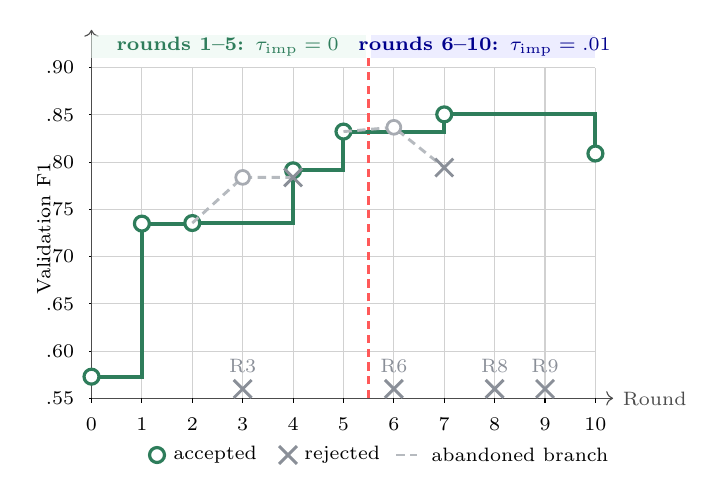
\begin{tikzpicture}[
  x=.64cm,y=12cm,
  accepted/.style={circle,draw=editgreen,fill=white,line width=1.15pt,minimum size=5.4pt,inner sep=0pt},
  rejected/.style={cross out,draw=fixgrey,line width=1.05pt,minimum size=5.4pt,inner sep=0pt},
  every node/.style={font=\scriptsize}
]
  \draw[black!18] (0,0) grid[xstep=1,ystep=.05] (10,.35);
  \draw[->,black!70] (0,0) -- (10.35,0) node[right] {Round};
  \draw[->,black!70] (0,0) -- (0,.39);
  \node[rotate=90] at (-.95,.18) {Validation F1};
  \foreach \x in {0,...,10} \draw (\x,0) -- +(0,-.005) node[below=2pt] {\x};
  \foreach \y/\lab in {0/.55,.05/.60,.10/.65,.15/.70,.20/.75,.25/.80,.30/.85,.35/.90}
    \draw (0,\y) -- +(-.04,0) node[left=2pt] {\lab};

  \fill[editfill,opacity=.55] (0,.36) rectangle (5.45,.385);
  \fill[blue!7] (5.55,.36) rectangle (10,.385);
  \node[font=\scriptsize\bfseries,text=editgreen] at (2.7,.3725)
    {rounds 1--5: $\tau_{\mathrm{imp}}=0$};
  \node[font=\scriptsize\bfseries,text=blue!55!black] at (7.8,.3725)
    {rounds 6--10: $\tau_{\mathrm{imp}}=.01$};
  \draw[densely dashed,red!65,line width=.9pt] (5.5,0) -- (5.5,.36);

  % Reported incumbent lineage.
  \draw[editgreen,line width=1.45pt]
    (0,.0229) -- (1,.0229) -- (1,.1849) -- (2,.1849) -- (2,.1855)
    -- (4,.1855) -- (4,.2413) -- (5,.2413) -- (5,.2823)
    -- (7,.2823) -- (7,.3005) -- (10,.3005) -- (10,.2591);

  \node[accepted] at (0,.0229) {};
  \node[accepted] at (1,.1849) {};
  \node[accepted] at (2,.1855) {};
  \node[accepted] at (4,.2413) {};
  \node[accepted] at (5,.2823) {};
  \node[accepted] at (7,.3005) {};
  \node[accepted] at (10,.2591) {};

  % Rejections use the compact baseline row convention of the Self-Harness
  % trajectory figure; their measured scores and context are in the side panel.
  \foreach \x/\lab in {3/R3,6/R6,8/R8,9/R9} {
    \node[rejected] at (\x,.010) {};
    \node[text=fixgrey,anchor=south] at (\x,.017) {\lab};
  }

  % Separately executed continuations, excluded from the reported lineage.
  \draw[fixgrey!62,densely dashed,line width=1.05pt]
    (2,.1855) -- (3,.2338) -- (4,.2338);
  \node[circle,draw=fixgrey!75,fill=white,line width=1pt,minimum size=5pt,inner sep=0pt] at (3,.2338) {};
  \node[rejected] at (4,.2338) {};

  \draw[fixgrey!62,densely dashed,line width=1.05pt]
    (5,.2823) -- (6,.2868) -- (7,.2442);
  \node[circle,draw=fixgrey!75,fill=white,line width=1pt,minimum size=5pt,inner sep=0pt] at (6,.2868) {};
  \node[rejected] at (7,.2442) {};

  % Marker legend, placed below the iteration axis as in Self-Harness.
  \node[accepted] at (1.30,-.060) {};
  \node[anchor=west] at (1.43,-.060) {accepted};
  \node[rejected] at (3.90,-.060) {};
  \node[anchor=west] at (4.03,-.060) {rejected};
  \draw[fixgrey!62,densely dashed,line width=1.05pt] (6.05,-.060) -- (6.45,-.060);
  \node[anchor=west] at (6.55,-.060) {abandoned branch};
\end{tikzpicture}
\end{minipage}%
\hfill
\begin{minipage}{.52\linewidth}
\centering\scriptsize
\setlength{\tabcolsep}{2.2pt}
\renewcommand{\arraystretch}{1.05}
\begin{tabularx}{\linewidth}{@{}lrrrrrX@{}}
\toprule
R & F1 & $\Delta$F1 & $\Delta$tok & Fail. & Dec. & What changed \\
\midrule
1  & .7349 & +.1620 & $-8.9\%$   & $23\to6$ & Prom. & emit user-ID pairs \\
2  & .7355 & +.0007 & $+11.7\%$  & $6\to1$  & Prom. & recover missing users \\
3  & .7838 & +.0483 & $-3.4\%$   & $1\to1$  & Rej.  & wrong-format regression \\
4  & .7913 & +.0558 & $-12.1\%$  & $1\to0$  & Prom. & confirm target categories \\
5  & .8323 & +.0410 & $+16.8\%$  & $0\to0$  & Prom. & correct detected errors \\
6  & .8368 & +.0045 & $-14.1\%$  & $0\to0$  & Rej.  & below revised $\tau_{\mathrm{imp}}=.01$ \\
7  & .8505 & +.0182 & $-33.8\%$  & $0\to0$  & Prom. & resolve count mismatch \\
8  & .8164 & $-$.0341 & $+56.5\%$  & $0\to1$  & Rej.  & format regression, +1 fail \\
9  & .6546 & $-$.1959 & $+665.7\%$ & $0\to7$  & Rej.  & token blowup, +7 fail \\
10 & .8091 & +.0128 & $-11.0\%$  & $0\to0$  & Prom. & rebuild after corrections \\
\bottomrule
\end{tabularx}
\end{minipage}
\caption{OOLONG-Pairs optimization trajectory (left) and the full per-round
record it summarizes (right). Changes are relative to that round's incumbent;
terminal failure counts are out of 72 attempts. Dark-green circles and the
step line denote accepted candidates on the reported incumbent lineage; gray
crosses in the row above the iteration axis denote rejected candidates.
Light-gray dashed traces show two abandoned exploratory continuations, found
by checking every sibling experiment directory in this lineage.}
\label{fig:optimization-trajectory}
\end{figure*}

% Diff-card primitives for fig:final-surface-edits: a full-width shaded row
% per logical line, "+" for appended text in that round's own color, plain
% (phantom-indented to match) for text retained verbatim from H0.
% Colorbox-around-parbox (not soul's \hl) so the shading spans the whole
% card width even when a line wraps. Round-to-text attribution verified
% against the real harness.json snapshots at each round (not the short
% behavioral_change summaries, which omit one of round 10's two insertions).
\newcommand{\diffsame}[1]{%
  \noindent\parbox{\dimexpr\linewidth-2\fboxsep\relax}{\ttfamily\small\phantom{+ }#1}\par\vspace{2pt}}
\newcommand{\diffadd}[2]{%
  \noindent\colorbox{#1}{\parbox{\dimexpr\linewidth-2\fboxsep\relax}{\ttfamily\small+\ #2}}\par\vspace{2pt}}
% Round-number badge for card titles: black text, background matching that
% round's own row fill color (not colored text) -- tight padding so it reads
% as a small tag rather than a full-size colorbox.
\newcommand{\rbadge}[2]{{\setlength{\fboxsep}{1.5pt}\colorbox{#1}{\textcolor{black}{#2}}}}

\begin{figure*}[p]
\centering
\setlength{\fboxsep}{4pt}
\begin{tcolorbox}[
  enhanced, colback=white, colframe=black!35, boxrule=0.5pt,
  arc=2pt, left=3pt, right=3pt, top=3pt, bottom=4pt,
  colbacktitle=black!8, coltitle=black, fonttitle=\bfseries\small,
  title={S2---decomposition instruction (promoted round \rbadge{r4fill}{4})}
]
\diffsame{Start by probing `context' to understand what you have, then decide how the task breaks into steps.}
\diffadd{r4fill}{Before selecting target categories, re-read the task question from `context' to identify which categories are required.}
\diffadd{r4fill}{Store the required categories in a variable and print them to confirm they match the task.}
\end{tcolorbox}

\vspace{4pt}
\begin{tcolorbox}[
  enhanced, colback=white, colframe=black!35, boxrule=0.5pt,
  arc=2pt, left=3pt, right=3pt, top=3pt, bottom=4pt,
  colbacktitle=black!8, coltitle=black, fonttitle=\bfseries\small,
  title={S3---execution instruction (cumulative promoted edits from rounds
    \rbadge{r1fill}{1}, \rbadge{r2fill}{2}, \rbadge{r5fill}{5}, and
    \rbadge{r10fill}{10})}
]
\diffsame{On each turn, run one block of code, print what you need to see, and build the result up in REPL variables.}
\diffadd{r1fill}{After classifying questions, generate the required user-ID pairs and output them in the format (user\_id\_1, user\_id\_2), one per line.}
\diffadd{r10fill}{When generating pairs from two user sets, skip pairs where the two user IDs are equal (a user cannot pair with itself).}
\diffadd{r2fill}{After classifying, verify that all users with entity or human being questions are captured. If any user appears to be missing, reclassify their questions.}
\diffadd{r5fill}{If you detect a classification error (e.g., a user's question count doesn't match the expected pattern), reclassify the affected questions before proceeding.}
\diffadd{r10fill}{After any reclassification, you MUST rebuild the user-to-category mapping and regenerate all pairs from scratch using the updated classifications. Do not reuse a previously computed user set or pair list after any classification change.}
\end{tcolorbox}

\vspace{4pt}
\begin{tcolorbox}[
  enhanced, colback=white, colframe=black!35, boxrule=0.5pt,
  arc=2pt, left=3pt, right=3pt, top=3pt, bottom=4pt,
  colbacktitle=black!8, coltitle=black, fonttitle=\bfseries\small,
  title={S4---verification instruction (promoted round \rbadge{r7fill}{7})}
]
\diffsame{Check your candidate answer before setting `answer["ready"] = True'.}
\diffadd{r7fill}{If you compute an expected count (e.g., of pairs, users, or classifications) and it does not match the actual count, do not submit until the discrepancy is resolved.}
\diffadd{r7fill}{Print the source of the discrepancy: which users or classifications differ between the expected and actual sets.}
\diffadd{r7fill}{Correct the underlying issue (e.g., reclassify affected questions, regenerate pairs) and re-verify before submitting.}
\end{tcolorbox}

\caption{Full retained field values for every surface changed in the frozen
round-10 harness, shown as a diff against the initial $H_0$ text: a plain line
is retained verbatim from $H_0$; a ``+'' line is new text, colored by the
round that added it (round number colored to match in each card's title).
S3 draws on four rounds, each shown in its own color; round 10 contributes
two separate insertions, one in the middle of the existing text and one at
the end, not a single trailing append. Every edit to these three surfaces was
a pure addition -- no span of the original text was altered or removed, so
no ``-'' lines appear anywhere. Unlike Figure~\ref{fig:optimization-trajectory},
this figure does not summarize the edits: it reproduces the full text from
the saved harness artifacts, diffed directly against the real per-round
harness snapshots (not the short per-candidate change summaries, which omit
one of round 10's two insertions).}
\label{fig:final-surface-edits}
\end{figure*}


Figure~\ref{fig:optimization-trajectory}'s side panel also demonstrates why
this run is not a Pareto-aware optimizer. Round 6 improves every displayed
objective (F1, tokens, failures) but is rejected by the scalar threshold,
while round 7 is promoted despite a 65.8\% provider-cost increase (its token
count falls 33.8\%). Applying Equation~\ref{eq:pareto-audit} to the available
round-level objectives, round 6 dominates its incumbent, whereas round 7 and its incumbent are
non-dominated because quality and tokens improve but cost worsens. The scalar
gate therefore produces \textbf{opposite decisions to the Pareto relation in
both rounds}. The appropriate claim is \emph{post hoc Pareto evaluation of a
constrained quality optimizer}.

\subsection{Pareto-Aware Frozen Length Audit}

\begin{table}[ht]
\centering\small
\setlength{\tabcolsep}{3.5pt}
\begin{tabular}{@{}lrrrrr@{}}
\toprule
Method & F1 & Tokens & Cost & Fail. & Instab. \\
\midrule
\hzero{}      & .6967 & 53.55M & \$2.788 & 6 & .2289 \\
\hzerostar{}  & .7248 & \textbf{26.72M} & \textbf{\$1.733} & 6 & .2048 \\
\shrlm{}      & \textbf{.7442} & 58.08M & \$2.915 & \textbf{2} & \textbf{.1630} \\
$\lambda$-RLM & .8472 &  1.05M & \$0.144 & 0 & .0321 \\
\bottomrule
\end{tabular}
\caption{Frozen 48-task OOLONG-Pairs test (96 runs/method). Tokens and cost are
totals; Fail. counts terminal failures. Instab. is the mean within-task absolute
difference between two attempts. $\lambda$-RLM is task-specific and its host
compute is unpriced. Bold marks the best generic harness on each objective.}
\label{tab:frozen48}
\end{table}

\begin{table}[ht]
\centering\scriptsize
\setlength{\tabcolsep}{3.2pt}
\renewcommand{\arraystretch}{1.02}
\begin{tabular}{@{}llrrrr@{}}
\toprule
Method & Metric & 8K & 16K & 32K & Macro / total \\
\midrule
\hzero{} & F1 & .7891 & .6481 & .6529 & .6967 \\
 & Tokens & 19.03M & 20.99M & 13.52M & 53.55M \\
 & Cost & \$0.816 & \$1.071 & \$0.900 & \$2.788 \\
\addlinespace[2pt]
\hzerostar{} & F1 & .6504 & \textbf{.7591} & \textbf{.7649} & .7248 \\
 & Tokens & \textbf{10.39M} & \textbf{8.81M} & \textbf{7.53M} & \textbf{26.72M} \\
 & Cost & \textbf{\$0.496} & \textbf{\$0.529} & \textbf{\$0.708} & \textbf{\$1.733} \\
\addlinespace[2pt]
\shrlm{} & F1 & \textbf{.8185} & .7142 & .7000 & \textbf{.7442} \\
 & Tokens & 18.07M & 22.40M & 17.61M & 58.08M \\
 & Cost & \$0.725 & \$0.931 & \$1.259 & \$2.915 \\
\addlinespace[2pt]
$\lambda$-RLM & F1 & .8829 & .8440 & .8148 & .8472 \\
 & Tokens & 0.129M & 0.328M & 0.592M & 1.05M \\
 & Cost & \$0.016 & \$0.050 & \$0.078 & \$0.144 \\
\bottomrule
\end{tabular}
\caption{Per-length frozen results for all four conditions. Each cell reports
mean F1, total recorded tokens, or total provider cost. Each length contains
16 tasks and 32 runs per method; the final column is macro F1 or the total over
all 96 runs. Bold marks the best generic harness; $\lambda$-RLM is specialized
and its host computation is unpriced.}
\label{tab:frozen48-length}
\end{table}

On the frozen test (Tables~\ref{tab:frozen48}--\ref{tab:frozen48-length}), \hzerostar{} strictly dominates
\hzero{}: it has higher F1, about half the tokens, 38\% lower cost, equal
failures, and lower instability. \shrlm{} raises observed F1 by .0194 over
\hzerostar{} and reduces failures, but uses 117\% more tokens and costs 68\%
more; neither dominates the other. The paired task-bootstrap interval for the
F1 difference is $[-.0521,.0935]$. By length, \shrlm{}--\hzerostar{} is +.1680
at 8K (95\% CI $[.0352,.3143]$), $-.0450$ at 16K
($[-.1590,.0561]$), and $-.0649$ at 32K ($[-.1586,.0278]$). Relative to
\hzerostar{}, \shrlm{} uses \textbf{74\%, 154\%, and 134\% more tokens} and
costs 46\%, 76\%, and 78\% more at 8K, 16K, and 32K, respectively. Thus the
aggregate gain comes from the 8K stratum and does not establish monotonically
improving length generalization or a quality--resource dominance relation.

$\lambda$-RLM exceeds \shrlm{} by .1031 F1 (95\% CI $[.0580,.1534]$), with
positive differences in all three length strata. It also records no terminal
failures and costs \$0.016/\$0.050/\$0.078 across 8K/16K/32K, compared with
\shrlm{}'s \$0.725/\$0.931/\$1.259. This is strong evidence that task-specific
algorithmic structure matters. It is not a clean systems-cost dominance claim,
because its deterministic host work is excluded from provider accounting.

\subsection{Long-Context and Cross-Task Audits}

The 8K/16K/32K division applies only to the stratified frozen length test.
The following evaluations each have one fixed regime: nominal 262K context for
OOLONG-Pairs and a full 3,507-document candidate corpus for OBLIQ-Bench Math.

\begin{table}[ht]
\centering\small
\setlength{\tabcolsep}{4pt}
\begin{tabular}{@{}lrrrr@{}}
\toprule
Method & 262K F1 & Tokens & Cost & Fail. \\
\midrule
\hzero{}      & .5696 & \textbf{80.13M} & \$10.962 & 7 \\
\hzerostar{}  & .5923 & 80.53M & \textbf{\$9.154}  & \textbf{1} \\
\shrlm{}      & \textbf{.6307} & 87.95M & \$10.384 & 2 \\
$\lambda$-RLM & .7465 & 22.12M & \$4.816  & 0 \\
\bottomrule
\end{tabular}
\caption{Frozen 40-task, nominal 262K OOLONG-Pairs test (80 runs/method).
Bold marks the best generic harness on each objective.}
\label{tab:long}
\end{table}

The 262K test repeats the frontier pattern (Table~\ref{tab:long}). \shrlm{}
improves over \hzerostar{} by .0383 F1, but the 95\% interval
$[-.0417,.1212]$ crosses zero and resource use is higher. $\lambda$-RLM's
.1158 advantage over \shrlm{} is resolved ($[.0737,.1657]$).

\begin{table}[ht]
\centering\scriptsize
\setlength{\tabcolsep}{3.5pt}
\begin{tabular}{@{}lrrrr@{}}
\toprule
Method & NDCG@10 & Tokens & Cost & Wrong fmt. \\
\midrule
\hzerostar{} & \textbf{.1040} & 70.18M & \$3.965 & \textbf{7} \\
\hzero{} & .0850 & 51.11M & \textbf{\$2.485} & 18 \\
\shrlm{} & .0517 & \textbf{50.54M} & \$2.534 & 29 \\
\bottomrule
\end{tabular}
\caption{Cross-task transfer to the frozen 40-query, full-corpus OBLIQ-Bench
Math split (80 runs/method). Tokens and provider cost are totals; Wrong fmt.
counts unparsable final answers. \shrlm{} receives no OBLIQ feedback. Bold
marks the best value on each objective.}
\label{tab:obliq-transfer}
\end{table}

Transfer is negative (Table~\ref{tab:obliq-transfer}). Relative to
\hzerostar{}, the frozen round-10 harness decreases mean NDCG@10 by 50.2\%
($-.0522$, paired 95\% CI $[-.0914,-.0175]$) and raises wrong-format failures
from 7/80 to 29/80. This loss is resolved despite \shrlm{} using 28.0\% fewer
tokens and 36.1\% lower provider cost. \hzerostar{} also has higher observed
NDCG@10 than \hzero{} by .0190, although its interval
$[-.0051,.0447]$ crosses zero. Because no OBLIQ feedback enters the search,
the result provides a concrete counterexample to broad cross-task robustness
claims for the learned harness.

\section{Discussion and Conclusion}

The optimization run is successful as an engineering search: it discovers a
harness with much better adaptive validation behavior and fewer formatting
failures. It is not evidence that the final harness is unconditionally better.
Frozen evaluation instead identifies a quality--efficiency frontier, unresolved
quality differences between generic harnesses, a decisive advantage for a
task-specific algorithm, and negative transfer. Reproducible AI reporting should
therefore distinguish three objects: the adaptive optimization record, an
untouched frozen test, and the multi-objective deployment choice. Publishing all
attempts and failures changes the scientific conclusion from ``automatic harness
improvement'' to the narrower and better-supported finding: scalar-guided
self-harnessing can find useful trade-offs, but robust improvement requires an
external Pareto audit.

\section{Limitations and Future Work}
\label{sec:limitations}

The 48-task length test yields only 16 independent tasks per stratum, and its
confidence intervals remain wide. Provider sampling is not guaranteed to be
stationary across dates. The same model proposes and executes edits, so results
may not transfer to other model families. Diagnosis text is model judgment, not
causal proof. Validation was accessed adaptively, and the threshold change after
round five prevents a fully pre-registered interpretation. Cost covers recorded
provider charges only; it omits host-side computation, which particularly favors
the deterministic operations in $\lambda$-RLM. The OBLIQ study is a transfer
audit, not an independently optimized environment. Larger frozen tests, matched
wall-clock accounting, multiple optimizer seeds, and replication on other
models are the highest-value next steps.

\paragraph{Broader impacts.}
Harness optimization could reduce manual engineering and improve the use of
fixed models, but a benchmark pass does not measure safe deployment or resistance
to misuse. Automatically edited instructions may change behavior outside the
benchmark, and safety is not part of the current promotion gate. This study uses
public benchmark data and no human-subject experiment or deployed decision
system. Its audit also shows that optimizing quality can increase resource use,
so downstream users should choose from a disclosed frontier rather than deploy
the highest-scoring artifact by default.

% AAAI sets the bibliography style itself (aaai2027.bst) — no \bibliographystyle.
\bibliography{aaai27/references}

% Working-paper appendices follow the references. Keep the historical
% optimization appendix as a separate, unchanged record of the earlier design.
\clearpage
\appendix
% Shared implementation appendix. Both active papers include this file in full.
\section{Runtime and Initial Harness}
\label{app:surfaces}

The implementation described here is the repository's main branch at revision
\texttt{5ae009e9}, with both study configurations inspected on November 15,
2026. These are implementation specifications for the forthcoming
study, not experimental results. The study's eventual launch revision, frozen
configuration, split manifest, and initial/final harness hashes must accompany
its results.

\paragraph{Initialization.}
\hzero{} supplies a minimal REPL contract and generic instruction strings, a
disabled runtime policy, the default metadata formatter, empty helper and skill
libraries, and accepting answer middleware. \hzerostar{} replaces S1 with the
upstream-style system prompt, leaves S2--S5 empty, and enables the orchestrator
addendum. \texttt{H0*R}, a hand-written reference, additionally replaces
S1's recursive-call description and supplies a hand-authored S2 example. That
example distinguishes a bare completion from a child with its own REPL, splits
line-oriented input into batches of 300, requests label counts, merges counts in
Python, and retries a chunk after a parse failure. It was informed by development
observations. Optimization starts from \hzero{}, not from \texttt{H0*R}, so the
learned harness can be compared against the hand-written one rather than seeded
by it. The \texttt{initial} evaluation condition loads the exact
saved round-one harness rather than substituting a reference from today's
registry. Figure~\ref{fig:edit-surfaces} and Figure~\ref{fig:full-repl-contract}
show the sparse \hzero{} reference.

\paragraph{Execution contract.}
S1--S5 are concatenated into one system prompt; a clause referring to early turns
is guidance, not a separately timed host hook. Recursive \texttt{rlm\_query}
children below the depth limit receive their own REPL and the shared prompt.
Bare \texttt{llm\_query} calls and leaves at the recursion limit are completions,
without that REPL. Printed code output joins accumulated message history;
input-as-variable does not prevent code from printing input records. The normal
answer path uses the REPL answer dictionary, while iteration exhaustion can
invoke the runtime's final-answer fallback. Admission checks preserve specified
interfaces and caps, not a formal proof of arbitrary generated code's behavior.

% AAAI: full-width table* for the long per-surface descriptions.
\begin{table*}[t]
\centering\small
\renewcommand{\arraystretch}{1.12}
\begin{tabularx}{\textwidth}{@{}p{0.17\textwidth}X@{}}
\toprule
Surface & Editable payload, visible information, and execution scope \\
\midrule
S1: REPL contract & Full text replacement describing the environment/API; shared root/recursive-child prompt. \\
S2: Decomposition & Full text replacement guiding input inspection and decomposition; shared prompt, scoped to the current subtask. \\
S3: Execution & Full text replacement guiding parsing, calls, aggregation, and task predicates; shared prompt. \\
S4: Verification & Full text replacement guiding checks before submission; shared prompt, with no independent semantic oracle. \\
S5: Recovery & Full text replacement guiding actions after visible errors; cannot extend a terminated run or add host retries. \\
S6: Runtime policy & Dictionary with enabled flag, prompt/batch caps, depth, syntax-retry/count, and output-validation settings. Enforcement is root local except inherited depth. Width/length caps refuse work; syntax retry repeats the same prompt. \\
S7: Metadata & Root formatter function receiving bounded stdout and redacted variable types/lengths; preserves its declared output bound. It cannot inspect hidden variable values or the full call history. \\
S8: REPL helpers & One named function added/replaced in one root or child helper dictionary. Helpers execute only when called; the proposer must identify a caller and input/output contract. \\
S9: Answer middleware & Root function receiving answer text and redacted inventory; may accept transformed text or redirect with a nudge. It cannot inspect hidden records or classifications. \\
S10: Skills & One named text procedure added, replaced, or removed. A shared name/description index advertises it; its body matters only when loaded or forwarded. \\
\bottomrule
\end{tabularx}
\caption{Ten surfaces and their actual capabilities. Provider/model selection,
decoding/reasoning settings, verifiers, and experiment-owned caps are outside the
edit space. S8 spans two fields; a surface is not necessarily one builder.}
\label{tab:surfaces}
\end{table*}

\paragraph{Skills and token accounting.}
The S10 index enters the system prompt after S5. For a nonempty library the
runner installs \texttt{load\_skill(name)} in root and recursive-child REPLs.
The host merges a single-entry edit with the incumbent library, including
explicit removal. Limits are eight entries, 40 characters per name, 200 per
description, 4,000 per body, and 16,000 total. A loaded body stored only in a
variable need not be model visible. If printed or forwarded it incurs input
tokens, potentially on later turns while it remains in history. Neither loading
a body nor advertising it proves that its procedure was followed.

% Figure 1: the sparse reference harness H0 and its ten editable surfaces.
% AAAI: full-width figure* (code lines are too wide for one column); figure*
% only supports [t] placement in AAAI (stfloats is forbidden).
% Body only; the `harness' listing style, its colours, and \hzero live in the
% preamble of proposal.tex, matching how Figure_2.tex relies on the tikz styling
% defined there.
\begin{figure*}[t]
    \centering
    \begin{lstlisting}[style=harness, gobble=4]
    # shrlm/rlm_harness.py: the ten surfaces Self-Harness may edit (S1 to S10).
    
    # Condensed for visibility; the full literal appears in the appendix.
    MINIMAL_REPL_CONTRACT = """
    You are an RLM operating through a persistent Python REPL.
    Use `context`, flat or recursive LM calls, `SHOW_VARS()`, and `answer`.
    Execute one ```repl``` block per turn; print inspections and mark the
    answer ready only when complete. [Display-only condensation.]
    """
    
    def build_repl_contract() -> str:                                    # S1
        return MINIMAL_REPL_CONTRACT
    
    def build_decomposition_instruction() -> str:                        # S2
        return ("Start by probing `context` to understand what you have, "
                "then decide how the task breaks into steps.")
    
    def build_execution_instruction() -> str:                            # S3
        return ("On each turn, run one block of code, print what you need "
                "to see, and build the result up in REPL variables.")
    
    def build_verification_instruction() -> str:                         # S4
        return 'Check your candidate answer before setting `answer["ready"] = True`.'
    
    def build_recovery_instruction() -> str:                             # S5
        return ("If a sub-call errors or returns something you cannot use, "
                "adjust the approach and try again.")
    
    def build_runtime_policy() -> dict[str, Any]:                        # S6
        return {
            "enabled": False,
            "max_prompt_chars": None,
            "max_batch_width": None,
            "max_depth": None,
            "retry_on_syntax_error": None,
            "max_retries": None,
            "validate_sub_output": None,
        }
    
    def build_metadata(                                                  # S7
        stdout: str,
        repl_inventory: dict[str, tuple[str, int]],
        max_character_length: int = DEFAULT_MAX_CHARACTER_LENGTH,
    ) -> str:
        return default_metadata_builder(stdout, repl_inventory,
                                        max_character_length)
    build_metadata.declared_bound = DEFAULT_MAX_CHARACTER_LENGTH        # S7
    
    def build_repl_helpers() -> dict[str, Any]:                          # S8
        return {}
    
    def build_sub_repl_helpers() -> dict[str, Any]:                      # S8
        return {}
    
    def build_answer_middleware() -> AnswerMiddlewareFn:                 # S9
        return accept_answer
    
    @dataclass(frozen=True)
    class SkillEntry:                                                    # S10
        name: str          # REPL-safe identifier; index label
        description: str   # one line: when to consult it; enters the prompt
        body: str          # ordered steps; served verbatim by `load_skill(name)`
    
    def build_skills() -> list[SkillEntry]:                              # S10
        return []
    \end{lstlisting}
    \caption{Sparse reference harness \hzero{} and its ten editable surfaces,
    each a declared field or group of fields (S8 has two builders). The configured
    study starts from \texttt{H0*R}, described in Appendix~\ref{app:surfaces}.
    S1 is condensed for display; Figure~\ref{fig:full-repl-contract} gives the
    full \hzero{} S1 template. S10 advertises a name/description index and loads
    bodies on demand; token cost depends on exposure in conversation history or
    forwarding to children. Each admitted edit changes one surface, and a round
    may compose several edits on distinct surfaces into one measured candidate.}
    \label{fig:edit-surfaces}
\end{figure*}

% Appendix figure: exact, unabridged sparse H0 S1 template (not H0*R).
% Figure 1 intentionally contains a display-only condensation of this prompt.
% AAAI: full-width figure* (the prompt lines are too long for one column);
% figure* only supports [t] placement in AAAI (stfloats is forbidden).
\begin{figure*}[t]
    \centering
    \begin{lstlisting}[style=harness, gobble=4]
    MINIMAL_REPL_CONTRACT = textwrap.dedent(
        """\
        You are a Recursive Language Model (RLM): a language model whose prompt-related information lives in a Python REPL that you drive turn by turn. You will be queried turn-by-turn until you have an answer to the query.

        Available in the REPL:
        - `context`: the information related to the prompt (typically `str` or `list[str]`).
        - `llm_query(prompt: str, model: str | None = None) -> str`: a single sub-LLM completion.
        - `llm_query_batched(prompts: list[str], model=None) -> list[str]`: several sub-LLM completions in parallel; same order out as in.
        - `rlm_query(prompt, model=None)` / `rlm_query_batched(prompts, model=None)`: recursive RLM sub-calls. Fall back to `llm_query` / `llm_query_batched` when recursion is disabled.
        - `SHOW_VARS() -> str`: list every variable currently in the REPL.
        - `answer`: dict initialized to `{{"content": "", "ready": False}}`. To submit, set `answer["content"]` to the final answer and `answer["ready"] = True` inside a ```repl``` block.
        {custom_tools_section}

        Write code in ```repl``` blocks, one block per turn; the REPL persists across turns. The REPL is NOT a Jupyter cell - only `print(...)` output (stdout) is shown back to you between turns; a bare expression on the last line is silently discarded. REPL outputs over ~20K characters are truncated."""
    )
    \end{lstlisting}
    \caption{The complete sparse \hzero{} S1 source template, before placeholder
    formatting. Figure~\ref{fig:edit-surfaces} uses a display-only condensation.
    This is a reference contract, not the full initial prompt of the configured
    \texttt{H0*R} study; its upstream-style prompt, recursive-call change, S2
    example, and orchestrator addendum are specified in
    Appendix~\ref{app:surfaces}.}
    \label{fig:full-repl-contract}
\end{figure*}

\section{Mining, Diagnosis, and Evidence Selection}
\label{app:mining}

Final-answer verification supplies pass/fail and an outcome category. Eligible
failed runs are sent to a fixed-model attributor; passing runs and configured
environment-owned exclusions are not sent through failure attribution. Excluded,
unattributed, and rejected records remain visible in accounting. Each diagnosis
records an inferred mechanism, location and causal status, supporting operation
references, and uncertainty. Structural absence of recursion can be observed
directly; semantic correctness and root-versus-child causality are not implied
by final-answer scoring.

The attributor must distinguish skipped records, wrong or uncertain labels, and
incorrect aggregation or predicates. Missing answer elements alone do not prove
input loss. It must account for observed checks and repairs, and distinguish
missing evidence from evidence that an action was omitted. For
\texttt{incomplete\_coverage}, a structured basis records status, input scope,
loss observation, and counterevidence. Statuses \texttt{not\_established} and
\texttt{contradicted} normalize to \texttt{OTHER}/\texttt{UNATTRIBUTED}, rather
than authorizing a coverage edit. Host acceptance verifies schema, vocabulary,
field bounds, and resolvable references, not the truth of a causal explanation.
Attribution response attempts default to three; transport retries are separate.

\paragraph{Clustering and routing.}
Records cluster by exact agreement on
% AAAI: split over two lines so it fits the single column.
\[
\begin{aligned}
\phi(r)=(&\text{outcome cause},\ \text{recorded failing level},\\
          &\text{causal status},\ \text{mechanism}).
\end{aligned}
\]
The signature mixes observed outcomes with model-inferred fields; it is not a
verified causal label. Patterns rank first by distinct-instance support, then
actionability, then a deterministic signature tie-break. Attempt support is
recorded separately. Minimum support two is a flag, not automatic deletion.
Three representatives and a fixed actionability heuristic guide reading order:
weights are 0.4 causal status, 0.3 grounding availability, 0.2 known mechanism,
and 0.1 normalized-description homogeneity. The last term uses distinct text
strings, not semantic embeddings; the score is not a calibrated success
probability.

\begin{table}[t]
\centering\small
\begin{tabularx}{\linewidth}{@{}Xl@{}}
\toprule
Mechanism & Eligible surfaces (primary first) \\
\midrule
REPL contract misuse & S1, S9, S10, S4 \\
Task objective misinterpretation & S2, S3, S4, S10 \\
Whole-input subcall collapse & S2, S3, S10, S6 \\
Incomplete coverage & S2, S4, S3, S10 \\
Redundant decomposition & S2, S3, S10 \\
Misaligned unit & S2, S10 \\
Depth degradation & S3, S6, S2 \\
Insufficient recursion & S3, S2, S6 \\
Bare completion substituted for recursion & S3, S1, S10 \\
Premature termination & S4, S9, S3 \\
Skipped verification & S4, S9, S10 \\
Swallowed subcall error & S5, S3, S6 \\
Iteration budget exhaustion & S6, S3, S1, S10, S5$^{\dagger}$ \\
Unparsed child output & S7, S3, S5, S8$^{\dagger}$ \\
REPL execution fault & S8, S10, S3, S1, S5$^{\dagger}$ \\
Answer serialization failure & S9, S4, S10 \\
Lossy aggregation & S3, S4, S8$^{\dagger}$ \\
Unconsulted procedure & S10, S3, S2 \\
Other & S1--S10 \\
\bottomrule
\end{tabularx}
\caption{Human-defined, many-to-many routing (taxonomy 3.4.0).
An \texttt{UNATTRIBUTED} diagnosis has no eligible route, including when its
mechanism is Other. $\dagger$ denotes additional operation-evidence requirements.}
\label{tab:routes}
\end{table}

Conditional S8 eligibility requires a complete cited operation; unparsed child
output additionally requires child-response evidence. Conditional S5 eligibility
requires an observed error and a subsequent complete operation. These are
structural opportunities to intervene, not proof of successful recovery or an
effective proposed fix. Aggregation errors route to S3/S4 or supported S8;
S9 remains limited to answer-visible properties.

\paragraph{Bounded evidence.}
The attribution digest defaults to 12,000 characters. Proposal evidence defaults
to 32,000 characters, separately from the 12,000-character history budget.
These are component budgets, not a total prompt cap. A compact pattern inventory
is supplemented by up to $\min(k,4)$ expanded patterns, preferring distinct
actionable mechanisms before additional signatures/context. Inventory-only
patterns do not authorize proposals. Evidence follows cited child calls and
relevant parsing, merging, or filtering operations, with nearby input definitions,
consumers, and corrections. Whole code operations are retained where they fit;
required operations that cannot fit are omitted with scope markers rather than
presented as complete fragments. Outputs and prose may be shortened. A passing
contrast sharing operation names can be included when available. This improves
context for comparison but guarantees neither full causal context nor balanced
surface coverage.

\section{Proposal, Materialization, and History}
\label{app:proposal}

One response under \texttt{proposal-selection/v2} selects evidence-supported
pattern/surface interventions before supplying replacement payloads; these are
not separate selection and generation calls. Each admitted candidate occupies
one exact (pattern, surface) pair: the same pattern may be attacked on several
surfaces, and the same surface may carry edits for different patterns, but a
pair cannot be claimed twice. Rejected entries reserve nothing. At most $k$
candidates are admitted, with fewer or zero allowed. Every admitted candidate is
materialized as its own complete harness, the incumbent with one surface
changed; candidates are never composed with each other. Three short explanation
fields identify incumbent behavior, unresolved observed failure, and the change
at a specific operation, input, or trigger. Guidance asks whether the same
demonstrated failure could persist if the edit were followed perfectly, and
requires the change to be stated as a forcing rule, a concrete trigger the
model will actually meet on a real input, rather than as softer or more
emphatic phrasing. Repeating an existing instruction more emphatically, moving
it to another surface, or repairing an already-recovered fault is insufficient
without a substantive behavioral difference. Replacing a misleading example can
be the smallest effective change.

The general prompt asks which information must survive each operation and which
task conditions must the final computation enforce. It does not prescribe an
OOLONG-specific record-ID algorithm. Environment-provided API and answer
contracts remain authoritative. These instructions guide model judgment; they
are not deterministic tests of semantic novelty or correctness.

\paragraph{Repair and preflight.}
Response/schema attempts are bounded (default maximum eight), distinct from
task validations. When failed-member repair is invoked there is one repair
response, restricted to failed original patterns. It may select another eligible
unoccupied surface or withdraw an edit while retaining valid siblings unchanged;
it may not invent new patterns. Collision repair must choose a contender or
withdraw it, still enforcing one admitted candidate per (pattern, surface) pair.

For text under \texttt{literal-text/v1}, the model supplies literal instructions;
the host encodes formatting braces exactly once and restores the designated
custom-tools placeholder. S1--S5 replace full text, S6 replaces a policy
dictionary, S7/S9 supply functions with required interfaces, S8 edits one named
helper in one dictionary, and S10 edits one named library entry. Preflight checks
serialization and base hashes, an actual single-surface change, reserved
interfaces, caps, formatting, and selected smoke/answer fixtures. Environment
answer fixtures are synthetic contract examples, not validation tasks. Literal
no-op rejection does not detect every behaviorally redundant instruction.
Saved artifacts distinguish literal proposal text, encoded source/template, and
runtime rendering.

\paragraph{History and qualified progress.}
The archive retains attempts, admission/rejection reasons, screening ranks,
measured outcomes, and revision links. The bounded prompt summary prioritizes
recent rounds, the incumbent's promotion, relevant measured predecessors, and an
older promising direction when it fits. Mechanisms already attempted on more
than one surface are listed separately, so the proposer sees that moving the
same idea to a new surface has been tried. Revisiting an intervention requires a
resolvable predecessor reference and a stated substantive change to the operation
or joint hypothesis. Validation contributes aggregate scores, costs, sanitized
failure summaries, and observed activation; its raw traces and gold/answer dumps
are not forwarded to the proposer.

A rejected measured candidate can be marked potentially promising when a
comparable verifier-defined dense metric improves in its declared direction.
Definitions specify identity/version, direction, aggregation, precision, and
terminal-outcome values. Comparison also requires compatible verifier/protocol/
repetition settings and matching instance-attempt sets. Missing, unsupported, or
incomparable metrics remain \texttt{not\_assessed}. The label is qualified
evidence, not promotion or statistical significance; a simultaneous exact-pass
regression remains recorded. An identical rejected harness already measured
under the same incumbent can be skipped before new validation.

\paragraph{Observed behavior.}
Instrumentation reports root S6 syntax retries and S9 redirects, and S10 loads
across the traced call tree, with observation coverage. Missing coverage is
unassessed. The intended-behavior field remains \texttt{not\_assessed}: activation
does not establish compliance or task correctness. There is no general semantic
compliance detector for S1--S5, S7, or S8.

\section{Screening, Validation, and Stopping}
\label{app:validation}
\label{app:algorithm}

Let $H$ be the incumbent and $C_1,\dots,C_{k'}$ ($k'\le k$) the admitted
candidates, each $H$ with one surface replaced. Let $V$ be the held-out
validation tasks, stratified by optimization context length
$\ell\in\mathcal{L}$, and $V_s\subset V$ a small fixed screening subset. For
OOLONG-Pairs, $V_s$ is curated from held-out task IDs of known difficulty and
spans every length (one, two, and three instances at 8K, 16K, and 32K). For
OBLIQ it holds the hardest and a median-scoring validation query per pool size.
Other environments use a generic small subset. Validation tasks are never mined.

\paragraph{Promotion metric and rule.}
The configured metric is either the verifier-pass count or a verifier-owned
primary quality. Both study profiles use primary quality: pair-set F1 for
OOLONG-Pairs and NDCG@10 for OBLIQ, written $F$ below. For harness $X$ let
$\bar F_\ell(X)$ be its mean primary quality over the attempts in stratum $\ell$, and
$\Delta_\ell=\bar F_\ell(C)-\bar F_\ell(H)$. A candidate $C$ is accepted when
\begin{equation}
\Delta_\ell\geq-\tau_\ell\ \ \forall\ell\in\mathcal{L},\qquad
\bar\Delta=\tfrac{1}{|\mathcal{L}|}\textstyle\sum_{\ell}\Delta_\ell\geq\tau_{\mathrm{imp}},
\label{eq:promotion}
\end{equation}
with equality tolerated up to floating-point precision. The per-length margins
$\tau_\ell$ are calibrated by a nested bootstrap over the incumbent's own
held-out scores at the 95th percentile, so any one length can veto a candidate
whose macro mean improves. Under the pass-count metric there is no length axis,
and a single $\tau_{\mathrm{reg}}$ bounds the pass-count change. For each
configured resource metric $q$, the candidate mean must also lie in the
inclusive band $a_q\bar q(H)\leq\bar q(C)\leq b_q\bar q(H)$, with unbounded
endpoints permitted. Cost-band enforcement can be disabled, in which case the
band is still recorded. An optional list of candidate-owned terminal failure
causes may not become more frequent than under $H$. Per-profile values are in
Table~\ref{tab:study-settings}; neither profile constrains sub-calls. Under the
OOLONG-Pairs setting $\tau_{\mathrm{imp}}=0$, a candidate with $\bar\Delta=0$
that clears every $\tau_\ell$ promotes. This is a selection rule, not a significance
test or a guarantee of per-task improvement.

\paragraph{Screening tournament.}
If $k'\ge2$, $H$ and every $C_i$ are evaluated independently on $V_s$ with
$v_s<v$ attempts per task; the incumbent is run fresh on exactly $V_s$ so that
every comparison uses the same tasks and attempts. Each candidate is scored
against $H$ with Equation~\ref{eq:promotion} and ranked by $\bar\Delta$.
Candidates that were never scored (for example, over budget) sink below every
scored one, and ties break deterministically by candidate identifier. Screening
verdicts are written to a separate screening ledger and are never promotion
decisions. If $k'\le1$, the tournament is skipped and the single candidate (if
any) proceeds directly.

\paragraph{Re-attribution.}
If every screened candidate fails Equation~\ref{eq:promotion} on $V_s$, the
already-executed mining runs are attributed a second time into a separate
evidence bundle, with no new task rollouts. This targets attribution noise:
independent re-attributions of the same digest often disagree. The proposer
then produces a fresh candidate pool from that bundle, which is screened in the
same way. The retry happens at most once per round. If it yields no candidate,
the original ranking stands. If its pool is also screened out, its own ranking
is used.

\paragraph{Full validation.}
Only the top-ranked candidate $C^\star$ is evaluated on all of $V$ with $v$
attempts, alongside $H$. Its $v_s$ screening attempts on $V_s$ are copied into
this evaluation and only the remaining instance-attempts run. If $H$ has not
changed since an earlier round, its completed held-out runs are reused rather
than repeated. Screening runs never seed an incumbent baseline, because they
cover only $V_s$. Under F1 promotion with early stopping enabled, $H$ is
evaluated first and $C^\star$'s tasks are ordered by length. Once all
of a length's runs are complete and $\Delta_\ell<-\tau_\ell$, the remaining
runs are skipped and $C^\star$ is rejected. Early stopping changes cost, not
the rule: a candidate that completes is judged by
Equation~\ref{eq:promotion}. If $C^\star$ is rejected, the other screened
candidates are retired rather than validated in turn.

\paragraph{Refinement.}
A rejected $C^\star$ may still improve F1 on runs that produced a measurable
answer while failing more often with a terminal cause such as malformed
output. Refinement is considered when its F1 conditional on a measurable answer
exceeds $H$'s by at least $\delta_{\mathrm{ref}}$ on the same length strata
($\delta_{\mathrm{ref}}=0.02$). The configured terminal-cause failure rate is
recorded but does not gate admission. One repair generation then mines
$C^\star$ on the held-in tasks and attributes the failures. The proposer is
restricted to patterns whose verifier cause is in the configured set
(\texttt{wrong\_format}) and to a single edit applied to $C^\star$. The
resulting descendant is validated against the \emph{original} $H$ on the same
$V$ under Equation~\ref{eq:promotion}, reusing $H$'s held-out runs. The branch
has at most one generation and never recurses. Because it spends a full
mining-and-validation leg, the implementation waits for an explicit recorded
confirmation before running it. The decision is persisted either way.

\begin{quote}\small
\textbf{Inputs:} initial harness $H$, mining tasks $M$, validation tasks $V$ and
screening subset $V_s$, repetitions $m,v,v_s$, candidate ceiling $k$, round
ceiling $T$, patience $p$, and promotion settings. Initialize history and
no-promotion counter $z=0$.
\begin{enumerate}
\item For each round up to $T$, execute or resume $H$ on $M$ with $m$ attempts;
record final outcomes, traces, and available observations.
\item Diagnose eligible failures, cluster records, and select bounded evidence
and history. Propose, admit, and if needed repair up to $k$ single-surface
candidates on distinct (pattern, surface) pairs; preflight each one.
\item If at least two candidates load, screen $H$ and every candidate on $V_s$
with $v_s$ attempts and rank them. If all are screened out, re-attribute the
same mining runs once, propose a fresh pool, and re-screen.
\item Fully evaluate the top-ranked $C^\star$ (or the only candidate) and $H$
on $V$ with $v$ attempts, reusing $C^\star$'s screening runs and any stored runs
of an unchanged $H$, with optional per-length early stopping. An unscorable
baseline follows the experiment error path. If Equation~\ref{eq:promotion} and
the resource bands hold, set $H=C^\star$.
\item Otherwise, if refinement is enabled and admitted, run one confirmed repair
generation from $C^\star$ and apply the same rule to its descendant against $H$.
\item Persist screening and promotion ledgers, or the reason no comparison
occurred; update history. Set $z=0$ on promotion, otherwise $z=z+1$. Stop when
$z\geq p$.
\item Freeze the last incumbent; run separately specified final-evaluation
conditions. Do not retrospectively select a harness using test scores.
\end{enumerate}
\end{quote}

\paragraph{Failures, denominators, and resume.}
Candidate-owned execution errors can become failed attempts without terminating
the whole experiment. Configuration/operational/provider errors, cancellation,
memory or I/O failures, and observation-persistence failures may still propagate.
Complete comparisons require matching planned attempts; a partial baseline cannot
anchor promotion. The final-evaluation driver can retain completed sibling
results while reporting an incomplete or over-budget condition.

\begin{table}[t]
\centering\small
\begin{tabularx}{\linewidth}{@{}p{0.27\linewidth}X@{}}
\toprule
Recorded status & Treatment \\
\midrule
Completed correct/incorrect & Enters attempt denominator; only a verifier pass counts as success. \\
Completed execution/resource/format/filter failure & Enters denominator as a failure; dense terminal values follow the verifier definition. Partial usage/trace coverage remains labeled. \\
Missing/canceled attempt & Report separately, not as a fabricated measured zero. Incomplete validation cannot silently become a complete comparison. \\
Unscorable baseline & Persist evidence and stop/raise through the experiment error path; this is not a candidate rejection. \\
Resumed/cached completion & Reuse only with matching identity/contracts; not a new independent attempt or new spend. \\
\bottomrule
\end{tabularx}
\caption{Outcome accounting for optimization and final evaluation.}
\end{table}

\section{Experimental Protocol and Provenance}
\label{app:protocol}

\paragraph{Profiles.}
Optimization runs from
\path{configs/experiment_oolong_pairs_blended_openrouter_DeepSeekV4Flash.toml} and
\path{configs/experiment_obliq_bench_math_openrouter_DeepSeekV4Flash_blended_h0init.toml}
via \path{examples/run_experiment.py}. Final evaluation runs from
\path{examples/run_evaluation.py} on each experiment's frozen splits, with conditions
\texttt{b1} (\hzero{}), \texttt{h0\_star} (\hzerostar{}), \texttt{lambda\_rlm}, and
\texttt{sh\_rlm}. The configuration identity is hashed on first use, and any later
change to an identity-covered setting refuses to resume the experiment.

\paragraph{OOLONG-Pairs data and scoring.}
The dataset is \texttt{oolongbench/oolong-synth}, upstream validation partition,
\texttt{trec\_coarse}, revision
\path{f0d59eaf0febf130664cfceb710436c8e3216b2b}. For each nominal window (8K,
16K, 32K, and the test-only 262K), the loader selects the first two distinct
record collections, with a 50,000-row scan ceiling, and pairs each with task
IDs 1--20, giving 40 instances per window. Labels are removed from
model-visible records; gold user-pair sets are computed from the labeled
records and task predicates. Within each optimization window, roles are 8
mining, 8 validation, and 4 test instances. A further 8 are reserved for a
refinement promotion split that the current implementation does not use,
because refinement validates on the ordinary validation set. Role assignment
follows a curated task order rather than the raw seeded shuffle, so that
validation includes known-hard task IDs (11 and 18) as well as easier ones. All
40 262K instances are test-only.

The scorer extracts integer pairs and compares sets. Global pair order and
duplicate pairs do not affect set equality, but order within a pair is preserved:
the lower user ID must come first. A bracketed list or newline-separated pairs
are accepted. The explicit empty marker is ``No valid pairs found.''; literal
\texttt{[]} is not an empty answer. No parseable pair or marker is a format
failure. A correctly empty prediction against an empty gold set passes and has
precision/recall/F1 equal to one. These extraction and empty-set distinctions
are adaptations of the example scorer, not an unmodified upstream verifier.

Different predicates over the same record collection ask different aggregation
questions over identical records, and each window has only two collections. Test
results at the optimization windows therefore measure held-out task instances,
not unseen records. The 262K test uses larger, distinct collections that share
question texts with the shorter ones; it measures length generalization, not
wholly unseen source text. Stripping labels and adding task text changes actual
prompt lengths, so evaluation reports measured prompt sizes separately from the
nominal window labels.

\paragraph{OBLIQ-Bench Math data and scoring.}
The dataset is \texttt{dianetc/OBLIQ-Bench}, \texttt{analogues/math} subset,
revision \path{4ebee29f68ceeb62ca00bd73d5478acdd3cd7764}: 3,508 corpus problems,
151 queries, and binary relevance judgments. Each instance is a query, a
candidate pool, and instructions to end with a ranked list of at most ten
bracketed corpus IDs. The pool holds the query's gold problems plus random
negatives up to 200, 500, or 1,000 problems, sampled with a seed per query;
the query's own self-match IDs are excluded. Each pool size draws a
\emph{disjoint} set of queries rather than the same queries at three
difficulties. Test queries come from a frozen 40-query split used in earlier
full-corpus comparisons, and mining and validation queries come from the
remaining 111. Each pool size receives 8 mining, 8 validation, and 4 test
queries. The screening subset holds the hardest and a median-scoring validation
query per pool size, chosen from the round-one incumbent's validation scores.

The verifier takes the last \texttt{RANKED:} list in the answer, keeps the first
ten distinct IDs, and computes NDCG@10. A missing list is a format failure, and
an explicit empty list is \texttt{no\_answer}. NDCG@10 of at least 0.9 counts as
a pass. Below that, the failure is labeled incomplete, spurious, or mixed by
whether gold IDs are missing, extra IDs are present, or both. Because all
judgments share one relevance grade, a prediction equal to the gold set scores
1.0 regardless of order.

\paragraph{Model, caps, and concurrency.}
All three roles use \texttt{deepseek/deepseek-v4-flash} through OpenRouter with
temperature 0, top-$p$ 0.95, and an output-token cap of 8,192. The provider's
default reasoning mode is enabled, without guaranteeing returned reasoning.
Each run is capped at depth three, 3,600 seconds, and \$2. OOLONG-Pairs allows 45
iterations plus a three-iteration, 600-second finalization window in which only
answer submission remains available. OBLIQ allows 30 iterations. Each validation
or screening subject, including the incumbent, has a \$100 cumulative budget.
Concurrency settings (mining, screening, and validation workers) do not change
any repetition count. Final evaluation uses three attempts per task per
condition.

The $\lambda$-RLM condition is identified by its method kind, reconstruction
version, upstream revision, and source hash; it is not an unmodified released
implementation for either environment. Model/deployment, rendered prompts,
source/configuration snapshots, split IDs/hashes, exact edit payloads, harness
lineage, and analysis versions belong in the study artifacts. Freezing these
before a run does not by itself constitute preregistration. Previously inspected
development or test material must retain its exposure history if later used to
support a result.

\section{Measurement, Cost, and Saved Observations}
\label{app:measurement}
\label{sec:cost}

\paragraph{Quality and surface activity.}
Exact pass is set equality, not rounded F1 equal to one. OOLONG-Pairs stores
per-attempt precision, recall, and F1 to three decimals; reported mean F1 averages
recorded attempt values, including verifier-declared zeros for completed runtime,
resource, format, and content-filter failures. It is macro averaging across
attempts, not pooled pair-level micro-F1. Missing/extra counts are reported only
where available, with coverage, rather than filling absent diagnostics with zero.
OBLIQ-Bench Math stores per-attempt NDCG@10 to three decimals, with format and
empty-answer failures scored zero; its pass rule is NDCG@10 at least 0.9.
Other environments supply their own metric definitions or remain unassessed.

Surface activity distinguishes submitted, admitted, evaluated, and promoted
edits, and records each candidate's screening rank separately from its
promotion decision. Because candidates are never merged, a promoted edit is the
whole measured difference from its incumbent; screened-out and retired
candidates carry only screening-subset estimates. Per-round quality plots use the freshly measured
candidate on promotion and freshly measured incumbent otherwise; a round without
a measurement is missing, not a zero or a carried-forward score. Environment
labels come from the configuration. Trace summaries can report depth, call
counts, and the implemented whole-input-subcall proxy: maximum descendant prompt
characters divided by root prompt characters exceeds 0.8. Its denominator is
walkable runs, passing and failing, with unwalkable runs separate; it is neither
a token ratio nor proof of meaningless decomposition.

\paragraph{Cost.}
An ordinary completed round with $k'\ge2$ loaded candidates schedules at most
\begin{equation}
N_{\mathrm{round}}=m n_{\mathrm{in}}
+(k'+1)\,v_s n_s
+\underbrace{v n_{\mathrm{ho}}}_{H}
+\underbrace{(v n_{\mathrm{ho}}-v_s n_s)}_{C^\star}
\label{eq:round-cost}
\end{equation}
task attempts, where $n_s=|V_s|$. The incumbent term is zero when an unchanged
incumbent's held-out runs are reused, and per-length early stopping can shorten
the $C^\star$ term. With $k'\le1$ there is no screening term and the candidate
runs all $v n_{\mathrm{ho}}$ attempts. A re-attribution adds one more screening
pool, at most $(k+1)v_s n_s$. An admitted, confirmed refinement adds
$m n_{\mathrm{in}}+v n_{\mathrm{ho}}$, with the incumbent's runs reused.
Both blended profiles have $n_{\mathrm{in}}=n_{\mathrm{ho}}=24$ across three
sizes, $m=2$, $v=3$, $k=4$, $v_s=1$, and $n_s=6$, so a full round schedules
$48+30+72+66=216$ attempts, or 144 when the incumbent is reused. OBLIQ disables
early stopping, re-attribution, and refinement, so its rounds have no further
terms. No admitted candidate means no screening or validation leg. Final
evaluation runs three attempts per task for each of the four conditions. With
12 short and 40 long OOLONG-Pairs test tasks that is $3\cdot52\cdot4=624$
attempts, and with 12 OBLIQ test queries it is $3\cdot12\cdot4=144$. These are
scheduling counts, not measured results or provider-call counts. Root attempts
may issue many recursive/model requests. Attribution, proposal, repairs, and
operational retries also consume resources.

The spend breaker uses the per-response cost OpenRouter returns. Configured
rates of \$0.009 per million input tokens and \$1.28 per million output tokens,
OpenRouter's listed price when the profiles were written, feed only cost
projections; they are not a current market quote. Actual usage and its coverage will be reported separately from scheduling
projections. Task usage is not added again to a stage total
that already includes it. Breaker reservations are not billed spend; interrupted
or unreported requests can leave a lower bound, and the per-run budget is not a
guarantee of complete invoice accounting.

\paragraph{Provider-returned observations.}
Instrumented execution, mining, validation, final evaluation, attribution,
proposal/repair, recursive calls, compaction, and fallback paths save returned
response/reasoning observations separately from executable code and final
answers. References carry call IDs, paths, and hashes. Run traces point to
\path{<run_id>.llm_calls/<call_id>/}; attribution and proposal artifacts point to
their stage-specific \path{llm_calls/} directories. Started, response, and finished
events distinguish failed or interrupted calls. Cache hits retain source
provenance and do not add spend.

Availability is explicit: \texttt{returned}, \texttt{opaque\_only},
\texttt{not\_returned}, \texttt{unsupported\_client},
\texttt{legacy\_unavailable}, or \texttt{no\_response}. Returned content can be
text or a summary; this is not guaranteed access to full private reasoning.
Unknown reasoning-token counts stay unknown and are not added to reported output
usage again. Legacy traces cannot be backfilled with unreturned reasoning.
Observation artifacts are not automatically fed into attribution digests,
proposal evidence, or history. Ordinary assistant prose in a digest is a
different source. Observation persistence errors remain visible failures.

% AAAI: full-width table* (the version strings are too long for one column).
\begin{table*}[t]
\centering\small
\begin{tabularx}{\textwidth}{@{}Xl@{}}
\toprule
Contract & Version \\
\midrule
Taxonomy / capabilities & 3.4.0 / \texttt{surface-capabilities/v2} \\
Attribution prompt / validator / digest & 1.6.0 / 1.2.0 / 1.8.0 \\
Proposal prompt / validator & 4.3.0 / 4.2.0 \\
Proposal response / text & \texttt{proposal-selection/v2} / \texttt{literal-text/v1} \\
Evidence selector / diagnostic history & 4.3.0 / 2.1.0 \\
Compact history & \texttt{proposal-history/v3} \\
Validation / summary & \texttt{heldout-batch/v2} / \texttt{shrlm-validation-summary/v3} \\
Behavior / provider observations & \texttt{behavior-observations/v1} / \texttt{rlm-llm-observation/v1} \\
\bottomrule
\end{tabularx}
\caption{Contracts at the documented revision; archive the versions actually
used by the forthcoming run with its results.}
\end{table*}

\section{Optional Follow-up Studies}
\label{app:extensions}
\label{app:finetune}
\label{app:alignment}

Cross-environment transfer would require a separately specified target protocol
and completed evaluation. A weight-training comparison would require an available
trainable checkpoint, justified backbone matching, and measured compute; no
fine-tuning condition or hardware allocation is claimed for this hosted study.
Because each promotion measures one single-surface edit against its incumbent,
per-round outcomes already attribute measured gains to individual edits. An optional future
leave-one-surface-out study would revert a final surface to its starting value
and rerun the same evaluation; it would measure that final-state counterfactual,
not the marginal contribution of every historical edit overwritten along the way.
No such ablation has been completed here.

An optional safety probe could compare frozen harness states for changes in
refusal and harmful-answer behavior, motivated by work on
misevolution~\citep{shao2025misevolution}. The task gate does not measure these
outcomes, so improved benchmark behavior would not establish safe deployment.
Any probe would need its own data, scoring, and budget. Textual reasoning
instructions are editable; provider reasoning settings are experiment owned.

\providecommand{\sid}[1]{\textbf{\texttt{#1}}}
\providecommand{\hzero}{\ensuremath{\mathrm{H}_{0}}\xspace}
\providecommand{\hzerostar}{\ensuremath{\mathrm{H}_{0}^{*}}\xspace}
\providecommand{\shrlm}{\textsc{SH-RLM}\xspace}
\providecommand{\TODO}[1]{\textcolor{red}{[TODO: #1]}}
\providecommand{\verdict}[1]{\textsf{#1}}

\section{Preliminary Optimization Runs}
\label{sec:diag}

\emph{These runs predate the study in Section~\ref{sec:setup}. They use a
different backbone (DeepSeek-V3.2) and a development branch with three extra
mechanisms that are not part of the study configuration. They exercised the
loop and informed its design. They are reported for transparency, not as the
paper's results.}

Validation tells the loop \emph{whether} an edit beat its incumbent, but not
\emph{why}. The per-length regression margins $\tau_\ell$ are also constants,
calibrated once on another backbone (DeepSeek-V4-Flash). We add three
mechanisms that address these gaps and test them in two runs with DeepSeek-V3.2
on AWS Bedrock (\$0.62/\$1.85 per million input/output tokens; cost is computed
from list prices).

\subsection{Method additions}

\paragraph{Advisory post-mortem.}
After each round, the validated candidate is replayed on up to six failed
\emph{held-in} instances from the pattern it targeted, plus up to three that the
incumbent passed. Each replay is paired with the incumbent's mining trace on the
same instance. The host first labels each instance \emph{improved},
\emph{regressed}, or \emph{within range}: F1 must leave the incumbent's attempt
range by more than $0.05$ to count as a change. A fixed model then assigns each
edit one verdict, \verdict{confirmed}, \verdict{refuted},
\verdict{not\_activated}, \verdict{inconclusive}, or
\verdict{regressed\_protected}, with trace citations and a one-sentence lesson.
The host rejects any verdict that contradicts its own facts, for example
\verdict{confirmed} with no improved target. Lessons go only to the next
proposer. The post-mortem never affects promotion and never reads held-out data.

\paragraph{Self-calibrated margins.}
Let $Q_\ell\in[0,1]^{n\times a}$ hold the incumbent's held-out F1 scores at
length $\ell$, for $n$ instances and $a$ attempts each. A nested bootstrap
simulates two evaluations of the same harness. It resamples instances with
replacement, then attempts within each instance:
\begin{equation}
  \hat{\Delta}_\ell =
  \Bigl|\tfrac{1}{na}\textstyle\sum_{i,j} Q_\ell[I^{A}_i,J^{A}_{ij}]
      - \tfrac{1}{na}\sum_{i,j} Q_\ell[I^{B}_i,J^{B}_{ij}]\Bigr|.
  \label{eq:boot}
\end{equation}
Each round sets $\tau_\ell=q_{0.95}(\hat{\Delta}_\ell)$, using 5000 replicates.
Only the regression margins change; the improvement threshold stays at
$\tau_{\mathrm{imp}}{=}0$.

\paragraph{Borderline re-test.}
Sometimes exactly one length misses its margin, by at most $\beta{=}0.03$, and
that miss alone blocks acceptance. Both harnesses then get $a$ more attempts at
that length only. The length is re-decided on the pooled $2a$ attempts, against
a margin from \cref{eq:boot} drawn at $2a$ attempts. A round runs at most one
re-test.

\subsection{Study 1: small-scale run}
The first run was small: 3 held-in and 3 held-out instances per length, one
attempt each, a 1200\,s limit per run, and frozen $\tau_\ell$. It ran two
rounds, and both were vetoed at 16K despite higher macro F1
(\cref{tab:smoke}). The post-mortem rated the round-1 \sid{S8} helper
\verdict{not\_activated}: \emph{``Adding a helper is insufficient if the root
doesn't invoke it.''} Round 2's proposer then suggested ``verify and
\emph{correct} misclassifications, not just report them.'' The run also exposed
the noise: mining the \emph{same} harness twice gave held-in macro F1 0.853 and
then 0.598. That noise motivated the calibration and the re-test. The run cost
about \$11.

\begin{table}[t]
\centering\small
\begin{tabular}{@{}lccccl@{}}
\toprule
 & 8K & 16K & 32K & Macro & Decision \\
\midrule
\hzero & .276 & .470 & .446 & .397 & -- \\
R1: \sid{S8} & .598 & .321 & .494 & .471 & 16K veto \\
R2: \sid{S4}+\sid{S6} & .561 & .280 & .491 & .444 & 16K veto \\
\bottomrule
\end{tabular}
\caption{Study 1: held-out F1 from 3 runs per length. The 16K margin was
0.144. Round 1's 16K delta was $-.149$ and round 2's was $-.191$.}
\label{tab:smoke}
\end{table}

\subsection{Study 2: full-size run}
This run recreates the screening-tournament setup at full size: 8 held-in and 8
held-out instances per length, 2 mining and 3 validation attempts, $k{=}4$
screened candidates, and patience 3. The earlier V4-Flash run of the same setup
recorded no promotion in three rounds.

None of round 1's 48 mining runs or 144 validation runs produced the exact gold
pair set. A pass-count gate could therefore never promote, and graded F1 is
necessary. Mining mostly found \texttt{mixed\_set\_error} failures. Screening
ranked four single-surface candidates. The winner, \sid{S4}, adds an
instruction to spot-check users near a predicate's threshold against their
original questions.

The calibrated margins were 0.143/0.158/0.252, close to the frozen
0.144/0.144/0.244. The candidate
improved F1 at every length and was promoted (\cref{tab:val}). It also costs
$1.51\times$ more per run, because it makes more sub-calls. The post-mortem
nonetheless returned \verdict{refuted}. Of six failed held-in instances, two
improved and four did not move. Its lesson: \emph{``verification that only logs
findings without corrective feedback loops cannot fix classification
errors.''}

Round 2 mined 48 fresh runs on the round-1 harness. Two reached the exact gold
pair set, both on the same instance. All four first-pass candidates failed
screening, with macro deltas from $-0.111$ to $-0.222$. The loop then
re-attributed the same mining runs, with no new rollouts, and proposed again.
Two of the four new candidates passed screening. The top-ranked one, again
\sid{S4}, tells the model to reclassify a question and recompute the user sets
when it finds a mismatch, the corrective step that round 1's lesson found
missing.

The recalibrated margins were 0.150/0.129/0.173, so the 32K margin fell from
0.252 to 0.173 between rounds on the same model. The macro gain shrank from
+0.054 in screening to +0.013 in full validation (\cref{tab:val}). No length
crossed its margin, so no re-test ran, and cost per run was unchanged
($0.99\times$). The candidate was promoted, although none of the 144 validation
runs in this round produced the exact gold set. The post-mortem again returned
\verdict{refuted}. All three target instances stayed within the incumbent's
range, and the one protected instance fell from F1 1.0 to 0.934, which the
post-mortem attributes to a correct question being reclassified. Its lesson:
\emph{``Cross-checking classifications alone is insufficient.''} We stopped the
run after this round to keep budget for the long-context test, so no proposer
has used this lesson. The two rounds cost about \$94 in completed runs and
attribution, proposal and post-mortem calls.

\begin{table}[t]
\centering\small
\setlength{\tabcolsep}{7pt}
\renewcommand{\arraystretch}{1.2}
\begin{tabular}{@{}lcccc@{}}
\toprule
 & 8K & 16K & 32K & Macro \\
\midrule
\hzero & .700 & .746 & .609 & .685 \\
R1: \sid{S4}$^\dagger$ & .740 & .765 & .719 & .741 \\
\addlinespace
$\Delta$ & +.039 & +.019 & +.110 & +.056 \\
Veto line & $-$.143 & $-$.158 & $-$.252 & -- \\
\midrule
R2: \sid{S4}$^\dagger$ & .752 & .736 & .775 & .754 \\
\addlinespace
$\Delta$ & +.012 & $-$.029 & +.056 & +.013 \\
Veto line & $-$.150 & $-$.129 & $-$.173 & -- \\
\bottomrule
\end{tabular}
\caption{Study 2: held-out F1 from 24 runs per length (8 instances $\times$ 3
attempts). $^\dagger$Promoted. Each $\Delta$ is against that round's incumbent:
\hzero in round 1 and the R1 harness in round 2, whose validation runs were
reused. The veto lines are each round's self-calibrated margins.}
\label{tab:val}
\end{table}

\paragraph{Long-context test.}
We compare the frozen \shrlm harness with \hzerostar on the 256K OOLONG-Pairs
test set, which is 8$\times$ the longest optimization length. All four
conditions run on the same 9 tasks (3 per task group) with 3 attempts each, and all 9 ran
to completion (\cref{tab:long}). \shrlm scores higher on every task. Most of
the gap comes from how \hzerostar fails: 9 of its 27 runs end in
\texttt{wrong\_format} and score 0, and its runs average 592\,s, against
4094\,s for \shrlm. So \hzerostar mostly answers without classifying the
256K context question by question. \shrlm does that work, and its promoted
spot-check and reclassify steps still apply at this length. It costs
$1.5\times$ more per run.

Against the other two conditions the picture is weaker. \shrlm and \hzero are
tied: the difference is +.048, with a CI that includes 0, and \shrlm wins 6 of 9
tasks. \hzero also classifies question by question (4463\,s per run), but 2 of
its runs end in \texttt{wrong\_format} and 2 more are terminated. Most of
\shrlm's gain over \hzerostar therefore reflects \hzerostar's failures, not an
improvement over \hzero. $\lambda$-RLM is the strongest condition. It beats
\shrlm by .135 (CI excludes 0) and wins all 9 tasks, at $0.14\times$ the cost
per run and about 110\,s per run.
\Cref{fig:long} places the four conditions on quality and cost. $\lambda$-RLM is both the
most accurate and the cheapest condition, so it dominates the other three. \shrlm and
\hzero sit close together at the expensive end, and only the difference
against \hzerostar has a confidence interval clear of 0 in \shrlm's favor.

\begin{figure}[t]
\centering
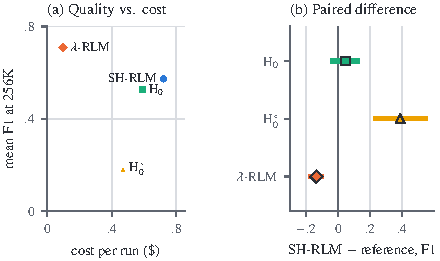
\includegraphics[width=\linewidth]{aaai27/figures/fig_long_context.pdf}
\caption{256K OOLONG-Pairs test (DeepSeek-V3.2; 9 tasks $\times$ 3
attempts per condition). (a)~Mean F1 against mean cost per run.
(b)~\shrlm minus each reference with task-level paired bootstrap 95\%
intervals; right of 0 favors \shrlm. Data as in \Cref{tab:long}.}
\label{fig:long}
\end{figure}

\begin{table}[t]
\centering\small
\begin{tabular}{@{}lccc@{}}
\toprule
256K & Tasks & Mean F1 & Cost/run \\
\midrule
\hzero & 9 & .526 & \$0.59 \\
\hzerostar & 9 & .185 & \$0.47 \\
$\lambda$-RLM & 9 & .708 & \$0.10 \\
\shrlm & 9 & .573 & \$0.72 \\
\bottomrule
\end{tabular}
\caption{Long-context generalization on matched tasks: 9 tasks $\times$ 3
attempts per condition, all complete. Paired difference +.388, 95\% bootstrap CI
[+.220, +.556]; \shrlm wins all 9 tasks. Against \hzero: +.048
[$-$.045, +.134]. Against $\lambda$-RLM: $-$.135 [$-$.187, $-$.088].}
\label{tab:long}
\end{table}

\paragraph{Discussion and limitations.}
The round-1 gain (+0.056) is below the bootstrap's noise level for macro F1
(0.108). Under $\tau_{\mathrm{imp}}{=}0$, the promotion is therefore a
selection decision, not a significant improvement. Round 2's gain (+0.013) is
further below its noise level (0.088), so its promotion is at most a tie-break
over the round-1 harness. That comparison also reuses the validation runs on
which the round-1 harness was selected, which may flatter the incumbent. The
post-mortems also suggest that neither edit worked through its stated
mechanism. The 256K test, the first independent check, does not show a gain over
\hzero, and $\lambda$-RLM outperforms both at a fraction of the cost. The 256K
set has only 9 tasks from two context windows. The bootstrap resamples instances
independently for the two harnesses, but validation compares them on the same
instances. The margins therefore overstate the noise, and a paired version
would tighten them. Each study is a single trajectory, with no run that
disables the post-mortem, so its benefit is not yet measured. Held-out sets are
small: 8 instances per length, drawn from two record collections. The code is
on branch \texttt{ELIAZ-LAST-SHOT} (commits \texttt{960fb7c6},
\texttt{2700c628}, \texttt{c1e3353b}; post-mortem first added in
\texttt{b961b4ce}).

\section{Reproducibility Record}
\label{app:repro}

Our retained experiment record contains the exact harness JSON for every
incumbent and candidate, immutable instance manifests, per-attempt JSONL records, execution
configuration, verifier output, trace paths, and SHA-256 trace digests. Runs use
accounting schema \texttt{shrlm-accounting/v2}. Each record stores instance ID,
attempt number, pass/fail cause, primary quality, input and output tokens,
provider cost, execution time, and whether usage is a lower bound. Tables in the
paper are computed from these records without dropping terminal failures. An
anonymized release artifact should preserve this structure and remove provider
credentials, local paths, and author-identifying metadata.

\paragraph{Frozen-test aggregation.}
For each method and task, we average its two attempts; the reported overall F1
is the equally weighted mean over tasks. Length-specific means use the 16 tasks
in that stratum. Total tokens and cost sum all attempts. A terminal failure is
an attempt whose cause is a resource termination or unparsable final format.
Paired bootstrap replicates sample task IDs with replacement and retain both
methods' attempts for each sampled task. Percentile endpoints use 200,000
replicates with a fixed analysis seed.

\paragraph{Artifact identities.}
The compared generic harnesses are the sparse round-zero harness, the pinned
upstream-prompt reference, and the promoted incumbent saved after round 10.
The specialized reference is the pinned $\lambda$-RLM reconstruction used in
both frozen OOLONG tests. The 48-task manifest is identical across all four
methods and contains 16 tasks at each nominal context length. The 262K manifest
contains 40 tasks, and the OBLIQ manifest contains 40 queries; each manifest is
reused verbatim across compared methods.

\paragraph{Decision semantics.}
The optimization objective is macro F1. Per-length non-regression and an
increase in \texttt{wrong\_format} are vetoes. Recorded token and provider-cost
changes are audit metrics, not a scalarized objective, and the configured cost
band is not enforced for this run. Rounds 1--5 use improvement threshold zero;
rounds 6--10 use .01, with round six recomputed after the change. No earlier
promotion is rewritten. These facts are necessary to reproduce the incumbent
sequence in Figure~\ref{fig:optimization-trajectory}.

\paragraph{What the artifact does not establish.}
OpenRouter does not guarantee replay-identical stochastic completions. The
artifact therefore supports verification of inputs, code paths, accounting,
and reported aggregation, but an independent rerun should be treated as a
replication rather than a bitwise reproduction. Provider charges exclude local
CPU work and should not be interpreted as complete energy or systems cost.


% Reproducibility checklist: if ReproducibilityChecklist.tex has its own
% \documentclass, compile and submit it separately instead of \input-ing it.
% \makeatletter
\@ifundefined{isChecklistMainFile}{
  % We are compiling a standalone document
  \newif\ifreproStandalone
  \reproStandalonetrue
}{
  % We are being \input into the main paper
  \newif\ifreproStandalone
  \reproStandalonefalse
}
\makeatother

\ifreproStandalone
\documentclass[letterpaper]{article}
\usepackage[submission]{aaai2027}
\setlength{\pdfpagewidth}{8.5in}
\setlength{\pdfpageheight}{11in}
\frenchspacing

\begin{document}
\fi
\setlength{\leftmargini}{20pt}
\makeatletter\def\@listi{\leftmargin\leftmargini \topsep .5em \parsep .5em \itemsep .5em}
\def\@listii{\leftmargin\leftmarginii \labelwidth\leftmarginii \advance\labelwidth-\labelsep \topsep .4em \parsep .4em \itemsep .4em}
\def\@listiii{\leftmargin\leftmarginiii \labelwidth\leftmarginiii \advance\labelwidth-\labelsep \topsep .4em \parsep .4em \itemsep .4em}\makeatother

\setcounter{secnumdepth}{0}
\renewcommand\thesubsection{\arabic{subsection}}
\renewcommand\labelenumi{\thesubsection.\arabic{enumi}}

\newcounter{checksubsection}
\newcounter{checkitem}[checksubsection]

\newcommand{\checksubsection}[1]{%
  \refstepcounter{checksubsection}%
  \paragraph{\arabic{checksubsection}. #1}%
  \setcounter{checkitem}{0}%
}

\newcommand{\checkitem}{%
  \refstepcounter{checkitem}%
  \item[\arabic{checksubsection}.\arabic{checkitem}.]%
}
\newcommand{\question}[2]{\normalcolor\checkitem #1 #2 \color{blue}}
\newcommand{\ifyespoints}[1]{\makebox[0pt][l]{\hspace{-15pt}\normalcolor #1}}

\section*{Reproducibility Checklist}

\vspace{1em}
\hrule
\vspace{1em}

\textbf{Instructions for Authors:}

This document outlines key aspects for assessing reproducibility. Please provide your input by editing this \texttt{.tex} file directly.

For each question (that applies), replace the ``Type your response here'' text with your answer.

\vspace{1em}
\noindent
\textbf{Example:} If a question appears as
%
\begin{center}
\noindent
\begin{minipage}{.9\linewidth}
\ttfamily\raggedright
\string\question \{Proofs of all novel claims are included\} \{(yes/partial/no)\} \\
Type your response here
\end{minipage}
\end{center}
you would change it to:
\begin{center}
\noindent
\begin{minipage}{.9\linewidth}
\ttfamily\raggedright
\string\question \{Proofs of all novel claims are included\} \{(yes/partial/no)\} \\
yes
\end{minipage}
\end{center}
%
Please make sure to:
\begin{itemize}\setlength{\itemsep}{.1em}
\item Replace ONLY the ``Type your response here'' text and nothing else.
\item Use one of the options listed for that question (e.g., \textbf{yes}, \textbf{no}, \textbf{partial}, or \textbf{NA}).
\item \textbf{Not} modify any other part of the \texttt{\string\question} command or any other lines in this document.\\
\end{itemize}

You can \texttt{\string\input} this .tex file right before \texttt{\string\end\{document\}} of your main file or compile it as a stand-alone document. Check the instructions on your conference's website to see if you will be asked to provide this checklist with your paper or separately.

\vspace{1em}
\hrule
\vspace{1em}

% The questions start here

\checksubsection{General Paper Structure}
\begin{itemize}

\question{Includes a conceptual outline and/or pseudocode description of AI methods introduced}{(yes/partial/no/NA)}
Type your response here

\question{Clearly delineates statements that are opinions, hypothesis, and speculation from objective facts and results}{(yes/no)}
Type your response here

\question{Provides well-marked pedagogical references for less-familiar readers to gain background necessary to replicate the paper}{(yes/no)}
Type your response here

\end{itemize}
\checksubsection{Theoretical Contributions}
\begin{itemize}

\question{Does this paper make theoretical contributions?}{(yes/no)}
Type your response here

	\ifyespoints{\vspace{1.2em}If yes, please address the following points:}
        \begin{itemize}
	
	\question{All assumptions and restrictions are stated clearly and formally}{(yes/partial/no)}
	Type your response here

	\question{All novel claims are stated formally (e.g., in theorem statements)}{(yes/partial/no)}
	Type your response here

	\question{Proofs of all novel claims are included}{(yes/partial/no)}
	Type your response here

	\question{Proof sketches or intuitions are given for complex and/or novel results}{(yes/partial/no)}
	Type your response here

	\question{Appropriate citations to theoretical tools used are given}{(yes/partial/no)}
	Type your response here

	\question{All theoretical claims are demonstrated empirically to hold}{(yes/partial/no/NA)}
	Type your response here

	\question{All experimental code used to eliminate or disprove claims is included}{(yes/no/NA)}
	Type your response here
	
	\end{itemize}
\end{itemize}

\checksubsection{Dataset Usage}
\begin{itemize}

\question{Does this paper rely on one or more datasets?}{(yes/no)}
Type your response here

\ifyespoints{If yes, please address the following points:}
\begin{itemize}

	\question{A motivation is given for why the experiments are conducted on the selected datasets}{(yes/partial/no/NA)}
	Type your response here

	\question{All novel datasets introduced in this paper are included in a data appendix}{(yes/partial/no/NA)}
	Type your response here

	\question{All novel datasets introduced in this paper will be made publicly available upon publication of the paper with a license that allows free usage for research purposes}{(yes/partial/no/NA)}
	Type your response here

	\question{All datasets drawn from the existing literature (potentially including authors' own previously published work) are accompanied by appropriate citations}{(yes/no/NA)}
	Type your response here

	\question{All datasets drawn from the existing literature (potentially including authors' own previously published work) are publicly available}{(yes/partial/no/NA)}
	Type your response here

	\question{All datasets that are not publicly available are described in detail, with explanation why publicly available alternatives are not scientifically satisficing}{(yes/partial/no/NA)}
	Type your response here

\end{itemize}
\end{itemize}

\checksubsection{Computational Experiments}
\begin{itemize}

\question{Does this paper include computational experiments?}{(yes/no)}
Type your response here

\ifyespoints{If yes, please address the following points:}
\begin{itemize}

	\question{This paper states the number and range of values tried per (hyper-) parameter during development of the paper, along with the criterion used for selecting the final parameter setting}{(yes/partial/no/NA)}
	Type your response here

	\question{Any code required for pre-processing data is included in the appendix}{(yes/partial/no)}
	Type your response here

	\question{All source code required for conducting and analyzing the experiments is included in a code appendix}{(yes/partial/no)}
	Type your response here

	\question{All source code required for conducting and analyzing the experiments will be made publicly available upon publication of the paper with a license that allows free usage for research purposes}{(yes/partial/no)}
	Type your response here
        
	\question{All source code implementing new methods have comments detailing the implementation, with references to the paper where each step comes from}{(yes/partial/no)}
	Type your response here

	\question{If an algorithm depends on randomness, then the method used for setting seeds is described in a way sufficient to allow replication of results}{(yes/partial/no/NA)}
	Type your response here

	\question{This paper specifies the computing infrastructure used for running experiments (hardware and software), including GPU/CPU models; amount of memory; operating system; names and versions of relevant software libraries and frameworks}{(yes/partial/no)}
	Type your response here

	\question{This paper formally describes evaluation metrics used and explains the motivation for choosing these metrics}{(yes/partial/no)}
	Type your response here

	\question{This paper states the number of algorithm runs used to compute each reported result}{(yes/no)}
	Type your response here

	\question{Analysis of experiments goes beyond single-dimensional summaries of performance (e.g., average; median) to include measures of variation, confidence, or other distributional information}{(yes/no)}
	Type your response here

	\question{The significance of any improvement or decrease in performance is judged using appropriate statistical tests (e.g., Wilcoxon signed-rank)}{(yes/partial/no)}
	Type your response here

	\question{This paper lists all final (hyper-)parameters used for each model/algorithm in the paper’s experiments}{(yes/partial/no/NA)}
	Type your response here


\end{itemize}
\end{itemize}
\ifreproStandalone
\end{document}
\fi

\end{document}
